% ---------------------------------------------------------------------
%                      DOCUMENTO DE EJEMPLO
%                    QUE UTILIZA LA PLANTILLA
%                    DE LA EDITORIAL DE LA UPV
%                  ADAPTADA A TESIS DOCTORALES POR 
%                       JUAN GARCIA MENDEZ
% ---------------------------------------------------------------------

\documentclass[nocrop, rm, english]{tesisUPV}

% Opciones de la clase 'tesisUPV'
%
% rm          - Tipo de letra roman
% sf          - Tipo de letra sans-serif
% crop        - Marcas de corte (cruz) 17x24 cm (+3 mm por los cuatro lados) centrada en una A4 
% nocrop      - Sin marcas de corte, respeta el tamaño 17x24 cm 
% nomathskip  - No se modifican las distancias de las ecuaciones 
%
% castellano  - La publicación está escrita en castellano
% valencia    - La publicació està escrita en valencià
% english     - La publicación está escrita en inglés

% Opcoines por defecto: rm, nocrop, english

% ---------------------------------------------------------------------
% Configuraciones presonalizadas 

% ---------------------------------------------------------------------
% ---------------------------------------------------------------------
% Configuración general

% For PDF/A documents, conflict with hyperref package not solved
%\usepackage[a-1b]{pdfx}

% To use "sen" as "sin" (sinus) for spanish/valencian maths
\newcommand{\sen}{\on{sen}}
\usepackage{csquotes}
% Quotes for valencian/catalen not defined, set to same as spanish
%\DeclareQuoteAlias{spanish}{catalan}

% Some general packages 
\usepackage{array,booktabs}
\usepackage{tabularx,longtable,multicol}
\usepackage{amssymb}

% ---------------------------------------------------------------------
% ---------------------------------------------------------------------
% Custom commands and packages JGM

% To use boldmath in headers
\usepackage{bm} 

% Change length between lines in math mode
\setlength{\jot}{12pt}

% Make the acronym list
\usepackage[acronym,shortcuts]{glossaries}

% Chapter 1
\newacronym{sm}{SM}{Standard Model}
\newacronym{cr}{CR}{Cosmic Ray}
\newacronym{cmb}{CMB}{Cosmic Microwave Background}
\newacronym{pmns}{PMNS}{Pontecorvo-Maki-Nakagawa-Sakata matrix for lepton mixing}
\newacronym{gzk}{GZK}{Greisen-Zatsepin-Kuzmin}

\newacronym{snr}{SNR}{Shell-type Supernova Remnant}
\newacronym{pwne}{PWNe}{Pulsar Wind Nebulae}
\newacronym{xrb}{XRB}{X-Ray Binary}
\newacronym{grb}{GRB}{Gamma-Ray Burst}
\newacronym{agn}{AGN}{Active Galactic Nucleus}

\newacronym{cc}{CC}{Charged Current}
\newacronym{nc}{NC}{Neutral Current}

\newacronym{pmt}{PMT}{Photomultiplier Tube}
\newacronym{om}{OM}{Optical Module}
\newacronym{dom}{DOM}{Digital Optical Module}
\newacronym{du}{DU}{Detection Unit}

\newacronym{dumand}{DUMAND}{Deep Underwater Muon And Neutrino Detector}
\newacronym{amanda}{AMANDA}{Antarctic Muon And Neutrino Detector Array}
\newacronym{nestor}{NESTOR}{Neutrino Extended Submarine Telescope with Oceanographic Research}
\newacronym{nemo}{NEMO}{Neutrino Ettore Majorana Observatory}
\newacronym{p-one}{P-ONE}{Pacific Ocean Neutrino Experiment}
\newacronym{trident}{TRIDENT}{TRopIcal DEep-sea Neutrino Telescope}
\newacronym{b-gvd}{Baikal-GVD}{Baikal Gigaton Volume Detector}
\newacronym{ic}{IceCube}{IceCube experiment}
\newacronym{sk}{Super-K}{Super-Kamiokande experiment}
\newacronym{orca}{ORCA}{Oscillation Research with Cosmics in the Abyss}
\newacronym{arca}{ARCA}{Astroparticle Research with Cosmics in the Abyss}


% Chapter 2

\newacronym{sl}{SL}{Single-Line (event)}

\newacronym{ai}{AI}{Artificial Intelligence}
\newacronym{dl}{DL}{Deep Learning}
\newacronym{ml}{ML}{Machine Learning}
\newacronym{tl}{TL}{Transfer Learning}

\newacronym{cnn}{CNN}{Convolutional Neural Network}
\newacronym{dcn}{DCN}{Deep Convolutional Network}
\newacronym{ffn}{FFN}{Feed-Forward Network}
\newacronym{mdn}{MDN}{Mixture Density Network}

\newacronym{pca}{PCA}{Principal Component Analysis}
\newacronym{relu}{ReLU}{Rectified Linear Unit}
\newacronym{elu}{ELU}{Exponential Linear Unit}
\newacronym{mle}{MLE}{Maximum Likelihood Estimation}
\newacronym{mae}{MAE}{Mean Absolute Error}
\newacronym{mse}{MSE}{Mean Squared Error}

\newacronym{cpu}{CPU}{Central Processing Unit}
\newacronym{gpu}{GPU}{Graphics Processing Unit}
\newacronym{io}{I/O}{Input/Output}
\newacronym{htc}{HTC}{High-Throughput Computing}
\newacronym{slurm}{SLURM}{Simple Linux Utility for Resource Management software}
\newacronym{in2p3}{IN2P3}{Institut National de Physique Nucléaire et de Physique des Particules}


% Chapter 3

\newacronym{mond}{MOND}{MOdified Newton Dynamics}
\newacronym{wmap}{WMAP}{Wilkinson Microwave Anisotropy Probe}

\newacronym{cdm}{CDM}{Cold Dark Matter}
\newacronym{macho}{MACHO}{MAssive Compact Halo Object}
\newacronym{bbn}{BBN}{Big Bang Nucleosynthesis}
\newacronym{pbh}{PBH}{Primordial Black Holes}

\newacronym{cp}{CP}{Charge-Parity}
\newacronym{qcd}{QCD}{Quantum ChromoDynamics}
\newacronym{susy}{SUSY}{SUperSYmmetric}
\newacronym{mssm}{MSSM}{Minimal Supersymmetric Standard Model}
\newacronym{lsp}{LSP}{Lightest Supersymmetric Particle}
\newacronym{lhc}{LHC}{Large Hadron Collider}
\newacronym{cern}{CERN}{Conseil Européen pour la Recherche Nucléaire}

\newacronym{sd}{SD}{Spin-Dependent}
\newacronym{si}{SI}{Spin-Independent}

\newacronym{tpc}{TPC}{Time Projection Chamber}

\newacronym{ams}{AMS}{Alpha Magnetic Spectrometer}
\newacronym{hess}{HESS}{High Energy Stereoscopic System}
\newacronym{magic}{MAGIC}{Major Atmospheric Gamma-ray Imaging Cherenkov}
\newacronym{xenon}{XENON}{XENON experiment}
\newacronym{lux}{LUX}{Large Underground Xenon experiment}
\newacronym{zeplin}{ZEPLIN}{ZonEd Proportional scintillation in LIquid Noble gases}
\newacronym{lz}{LZ}{LUX-ZEPLIN experiment}
\newacronym{darkside}{DarkSide}{DarkSide direct-detection experiment}
\newacronym{pico}{PICO}{PICO bubble chamber experiment}
\newacronym{cresst}{CRESST}{Cryogenic Rare Event Search with Superconducting Thermometers}
\newacronym{supercdms}{SuperCDMS}{Super Cryogenic Dark Matter Search}
\newacronym{EDELWEISS}{EDELWEISS}{Expérience pour DEtecter Les WIMPs En SIte Souterrain}

\newacronym{wimpsim}{WimpSim}{WIMP Simulation software}
\newacronym{darksusy}{DarkSUSY}{Supersymmetric Dark Matter simulation software}

\makeglossaries
% Make the acronym list print as a chapter-level heading
\setglossarysection{chapter}
% Bold acronym names, keep descriptions normal
\newglossarystyle{longbold}{%
  \setglossarystyle{long}% base on the standard 'long' style
  \renewcommand*{\glsnamefont}[1]{\textbf{##1}}% make the entry name bold
}

% Para incluir la portada como PDF (y otros PDFs si fuera necesario)
\usepackage{pdfpages}

% Para usar multirow in tables
\usepackage{multirow, makecell}

% Para poner celdas de colores en las tablas
\usepackage[table]{xcolor}  % Permite usar \cellcolor en tablas
\usepackage{colortbl}       % Opcional, pero mejora compatibilidad con tablas

% Comandos para notas y ocultar bloques de texto
\newcommand{\hide}[1]{}

% Para poner notas en el texto
\usepackage[colorinlistoftodos,prependcaption]{todonotes}
\newif\ifdraft

%\drafttrue   % pon \draftfalse para ocultarlos en la versión final
\draftfalse

\ifdraft
  \newcommand{\juan}[1]{\todo[color=blue!20,inline]{JGM: #1}}
  \newcommand{\salva}[1]{\todo[color=green!20,inline]{SA: #1}}
  \newcommand{\miquel}[1]{\todo[color=orange!25,inline]{MA: #1}}
\else
  \newcommand{\juan}[1]{}
  \newcommand{\salva}[1]{}
  \newcommand{\miquel}[1]{}
\fi

% Para usar la fuente \mathds
\usepackage{dsfont}

% Para rellenar trozos sin escribir
\usepackage{lipsum}

% Para usar lineas punteadas verticales en las tablas (|c:c|)
\usepackage{arydshln}

% Para usar subfiguras
\usepackage[labelfont=bf]{subcaption}
\renewcommand\thesubfigure{\Alph{subfigure}}

% Traducción del título del abstract
\addto\captionsenglish{\renewcommand{\abstractname}{Abstract}}
\addto\captionsspanish{\renewcommand{\abstractname}{Resumen}}
\addto\captionscatalan{\renewcommand{\abstractname}{Resum}}

% Entorno abstract personalizado tipo recomendado (como un capitulo)
\newenvironment{myabstract}{
  \chapter*{\abstractname}
  \addcontentsline{toc}{chapter}{\abstractname}
}{}

% Entorno abstract personalizado tipo report
\newenvironment{abstract}{
  %\cleardoublepage
  \clearpage
  \null\vfill
  \begin{center}%
    \bfseries \abstractname
  \end{center}}%
 {\vfill\null}

% Change subsubsections to not be in italic shape and being bold
\titleformat{\subsubsection}
  [hang]
  {\vspace{2ex}\raggedright\tolerance=10000\hyphenpenalty=10000}
  {\normalsize\bfseries\thesubsubsection}
  {1em}
  {\normalsize\bfseries}
  [\vspace{-0.75ex}]

% Change subsections to not be in italic shape
\titleformat{\subsection}
    [hang]
    {\vspace{1.5ex}\raggedright\tolerance=10000\hyphenpenalty=10000}
    {\fontsize{10.5}{12.5}\bfseries\thesubsection}
    {1em}
    {\fontsize{10.5}{12.5}\bfseries}
    [\vspace{-1ex}]

% ---------------------------------------------------------------------
% ---------------------------------------------------------------------
% ---------------------------------------------------------------------
% Bibliografía (modificar al gusto)

\usepackage[
	url      = false,
    eprint   = false,
    isbn     = false,
	style    = ieee, %numeric, %apa %authoryear
    citestyle = numeric-comp,
	hyperref = true,
	backref  = true,
	backend  = biber,
    sorting  = none,
    maxnames = 2,
    minnames = 2,
    giveninits = true,
	]{biblatex}

% To avoid reading the abstract in biber, avoid erros due to Unicode
\DeclareSourcemap{
  \maps[datatype=bibtex]{
    \map{
      % Remove abstract and languages to avoid bad printing
      \step[fieldset=abstract, null]
      \step[fieldset=language, null]
    }
    \map[overwrite=true]{
      % Only for Articles
      \pertype{Article}
      % Continue only if 'collaboration' exists (final):
      \step[fieldsource=collaboration, fieldtarget=author, final]
    }
  }
}


% ---------------------------------------------------------------------
% ---------------------------------------------------------------------
% Documento electrónico

\usepackage{imakeidx}
\makeindex


% Print boolean to change link colors. Set to true for printing, so links are black
\newif\ifprint
\printfalse
%\printtrue

% Define colors for links, internal references, etc
\colorlet{colorEnlace}{black}

\ifprint
    \colorlet{colorRef}{black}
    \colorlet{colorURL}{black}
\else
    \colorlet{colorRef}{blue}
    \colorlet{colorURL}{cyan}
\fi

% To allow URL breaks in many characters (just needed if overfull \hbox happens due to URLs)
% NOT TESTED
%\usepackage{xurl}

\usepackage[
	colorlinks,
    linkcolor=colorRef,
	citecolor=colorRef,
	urlcolor=colorURL,
    bookmarksnumbered,
	breaklinks,
	]{hyperref}

% Para usar \bookmarksetup % Debe estar siempre detras de hyperref
\usepackage{bookmark} % <- justo después de hyperref



% ---------------------------------------------------------------------
% ---------------------------------------------------------------------
% ---------------------------------------------------------------------
% ---------------------------------------------------------------------
% ---------------------------------------------------------------------
% ---------------------------------------------------------------------
% Below this point, I have not used anything of this.
% It was all declared by "editorial UPV", so it should work fine
% ---------------------------------------------------------------------
% ---------------------------------------------------------------------
% ---------------------------------------------------------------------
% ---------------------------------------------------------------------
% ---------------------------------------------------------------------
% ---------------------------------------------------------------------


% ---------------------------------------------------------------------
% ---------------------------------------------------------------------
% Expresión de unidades según el Sistema Internacional, monedas

\usepackage{eurosym}
\usepackage{siunitx}

\ifenglish
	\sisetup{output-decimal-marker={.}}
\else
	\sisetup{output-decimal-marker={,}}
\fi

\DeclareSIUnit[number-unit-product = {\;}] \EURO{\geneuro}


% ---------------------------------------------------------------------
% ---------------------------------------------------------------------
% Por compatibilidad con versiones anteriores de la plantilla
	
\newcommand{\incluyeGrafico}[2][]{\includegraphics[#1]{#2}} % Por compatibilidad

% ---------------------------------------------------------------------

\newcommand{\ingles}[1]{\textit{#1}}

% ------------------------------------------------------------------------

\usepackage{xspace}

\newcommand{\angles}[1]{\textit{#1}\/}
\newcommand{\miUrl}[1]{{\small%
	%\texttt%
	{\underline{#1}}}}

\newcommand{\matlabr}{{\sc Matlab}$^\circledR$\xspace}
\newcommand{\simulinkr}{\textit{Simulink}$^\circledR$\xspace}
\newcommand{\matlab}{{\textsc{Matlab}}\xspace}
\newcommand{\simulink}{\textit{Simulink}\xspace}

\newcommand{\scr}{\textit{script\/}\xspace}
\newcommand{\scrs}{\textit{scripts\/}\xspace}

% ------------------------------------------------------------------------

\definecolor{griset}{rgb}{.925, .925, .925}


\newsavebox{\mybox}
\newenvironment{parrafoDestacado}
    {%
    \fboxsep = 2ex
    \fboxrule = .4pt
    \begin{lrbox}{\mybox}%
    \begin{minipage}{.85\textwidth-2\fboxsep}\itshape\parskip=2ex
    }
    {%
    \end{minipage}
    \end{lrbox}%
    \begin{flushright}
        \colorbox{griset}{\usebox{\mybox}}%
        %\fcolorbox{black}{griset}{\usebox{\mybox}}%
    \end{flushright}
    }


% ------------------------------------------------------------------------
% Resumen del capítulo


\newsavebox{\myboxb}
\newenvironment{Resumen}
    {%
    \vspace*{-2.0cm}
    \fboxsep = 0pt
    \fboxrule = 0pt
    \begin{lrbox}{\myboxb}%
    \begin{minipage}{.85\textwidth}\itshape\parskip=2ex\parindent=2em
    }
    {%
    \end{minipage}
    \end{lrbox}%
    \begin{flushright}
        \usebox{\myboxb}%
    \end{flushright}
    \vspace{0.5cm}
    }

% ---------------------------------------------------------------------
% ---------------------------------------------------------------------
% Símbolos matemáticos

\newcommand{\on}{\operatorname}

% ---------------------------------------------------------------------
% ---------------------------------------------------------------------
% Teoremas y ejemplos

\ifcastellano
	\newtheorem{teorema}{\upshape\bfseries Teorema}[section]
	\newtheorem{lema}{\mdseries\scshape Lema}[section]
	\newtheorem{proposicion}{\upshape\bfseries Proposición}[section]
	\newtheorem{ejemplo}{\bfseries\scshape Ejemplo}[section]
\fi

\ifvalencia % Es mantenen els mateixos noms per compatibilitat, però l'autor els pot personalitzar
	\newtheorem{teorema}{\upshape\bfseries Teorema}[section]
	\newtheorem{lema}{\mdseries\scshape Lema}[section]
	\newtheorem{proposicion}{\upshape\bfseries Proposició}[section]
	\newtheorem{ejemplo}{\bfseries\scshape Exemple}[section]
\fi

\ifenglish
	\newtheorem{teorema}{\upshape\bfseries Theorem}[section]
	\newtheorem{lema}{\mdseries\scshape Lemma}[section]
	\newtheorem{proposicion}{\upshape\bfseries Proposition}[section]
	\newtheorem{ejemplo}{\bfseries\scshape Example}[section]
\fi

% ---------------------------------------------------------------------
% ---------------------------------------------------------------------

\newcommand{\FuenteEjemplos}{\small}

% ---------------------------------------------------------------------
% ---------------------------------------------------------------------
% Teoremas y ejemplos

\usepackage[most]{tcolorbox}


% ---------------------------------------------------------------------
% Ejemplo

\definecolor{colorFonsExemples}{rgb}{0.95,0.95,0.95}
\colorlet{colorFonsCapcaleraExemples}{black!65!white}

\newtcbtheorem[
	auto counter,
	number within = section,
	]{texemple}{Ejemplo}{
		enhanced jigsaw,
		breakable,
		pad at break* = 1mm,
		arc = 0.0mm,
		%
		sharpish corners,
		leftrule = 0pt, rightrule = 0pt,
		bottomrule = 0pt, toprule = 0pt,
		% borderline={0.4pt}{0pt}{black},
		% left=.5em,right=.5em,top=1ex,bottom=1ex, 
		%
		colback = colorFonsExemples,
		colframe = colorFonsExemples,
		description color = white,
		coltitle = white,
		colbacktitle = colorFonsCapcaleraExemples,
		fonttitle = \bfseries\sffamily\upshape\FuenteEjemplos,
		fontupper = \FuenteEjemplos,
		toptitle = 0.45ex, bottomtitle = 0.25ex,
		before skip = 4ex, after skip = 4ex,
		}{ejemplo}

\newenvironment{Ejemplo}[2]
	{
	\begin{texemple}{#1}{#2}
	\parskip = \separaParrafos % \separaParrafos está definido en la plantilla
	\parindent = \indentaParrafos % \indentaParrafos está definido en la plantilla
	% Per a les equacions normals
	\abovedisplayshortskip = -1.0ex plus 0ex minus 0.25ex
	\belowdisplayshortskip = 2.0ex plus 1ex minus 0.0ex	
	% Per a les equacions en varies l?nies
	\abovedisplayskip = -1.0ex plus 0ex minus 0.25ex
	\belowdisplayskip = 2.0ex plus 1ex minus 0.0ex
	}
	{
	\end{texemple}
	}

\newenvironment{enunciadoEjercicio}{\itshape}{} %\slshape

\newcommand{\finEjemplo}[1]{%
	\vspace{1ex}
	\begin{flushright}
		\slshape\FuenteEjemplos
		{Fin del ejemplo} \ref{ejemplo:#1}
		\hspace{1em}\textcolor{colorFonsCapcaleraExemples}{$\blacksquare$}
	\end{flushright}
	%
	\vspace{-1ex}
	}

		
% ---------------------------------------------------------------------
% Zona Grisa

\makeatletter
\newenvironment{zonaGrisa}{\begin{tcolorbox}[
		width = \textwidth-\@totalleftmargin,
		%left skip = .1\textwidth,
		enhanced jigsaw,
		sharpish corners,
		breakable,
		boxrule=0pt,
		leftrule = 0pt, rightrule = 0pt,
		left=1em,right=1em,top=3ex,bottom=1ex, 
		bottomrule=0pt,toprule=0pt,
		%borderline={0.0pt}{0pt}{black},
		colback=colorFonsSolucions,
		colframe=colorMarcSolucions,
		coltitle = black,
		fonttitle=\bfseries\upshape, %\scshape
		fontupper = \SelectFont\selectfont,
		before skip = 0ex, after skip = 4ex,
		]\parskip = 2ex}{\end{tcolorbox}}
\makeatother		
\usepackage{listings}

% \lstset{deletekeywords=[1]{structure}}

\lstset{
	language=[LaTeX]TeX,
	basicstyle=\small\ttfamily,         
	identifierstyle=,           
	commentstyle=\color[rgb]{.5,.5,.5},
	stringstyle=\color[rgb]{0,.5,0},
	tabsize=4,
	backgroundcolor = \color[rgb]{.96,.96,.96},
	rulecolor = \color[rgb]{.96,.96,.96},
	frame=single,
	framesep = 9pt,
	xleftmargin= 9pt,
	xrightmargin= 9pt,			
	classoffset=0,
	morekeywords={
		comando, marcaseccion, href,
		maketitle,
		signature, address, opening, closing, encl,
		appendix, include, includeonly, input,
		titlelabel, titleformat, thetitle, titlecontents, thecontentslabel, phantomsection, 
		addstarredchapter,
		nameref, indexIngles, printindex, 
		contentspage, titlerule, tableofcontents,
		dominitoc, minitoc,
		citet, citep, citeauthor, citeyear,
		sffamily, Large, familydefault, sfdefault,
		geometry, newgeometry, restoregeometry,
		autoref, nouppercase,
		tablename, figurename,contentsname,chaptername, bibname,
		colorlet,
		columncolor, rowcolor, ctable, LL, FL, ML, NN,
		toprule, midrule, cmidrule, arraybackslash, bottomrule, newcolumntype,
		chaptermark, thechapter,
		anchoPapel, margenInterior, ingles, comandoNuevo, SAC, SACs, todoDestacado, todoNormal,
		xspace, destacado, espacio, longLinea,
		labelitemi, labelitemii, labelitemiii, labelitemiv,
		labelenumi, labelenumii, labelenumiii, labelenumiv,
		mathcal,
		listoftables, listoffigures,
		columnbreak, clearpage,
		graphicspath, totalnumber, rotatebox, scalebox, resizebox, captionfo, subfloat,
		bottomnumber, topnumber,
		fbox, framebox, fcolorbox, colorbox, shadowbox, doublebox, ovalbox, Ovalbox, shadowsize,
		cornersize,
		setlength, floatstyle, newfloat, floatname, endfoot, endlastfood, endhead, endfirsthead,
		dfrac, tfrac, sen, tg, dif, overset, underset, text, eqref, nolimits,
		numberwithin, SI, si, num, euro, EURO, finEjemplo,
		pascal, kelvin, kilo, metre, meter, square, percent, kilogram, kilometre, per, second, hour, newton, volt, micro, centi, ifEPUB, Picture,
		theoremstyle, theoremheaderfont, theorembodyfont,
		includeonlyframes, frametitle, framesubtitle, mode, usetheme, usecolortheme, usefonttheme,
		useinnertheme, useoutertheme, note, setbeameroption, pgfpagesuselayout, pause, alert,
		structure, only, onslide, visible, invisible, uncover, alt, temporal, column, setlist,
		ifEBOOKPDF, ifenglish
		},
	keywordstyle=\color[rgb]{.45,.00,.00},
	classoffset=1,
	morekeywords={
		begin,
		end,
		chapter, section, subsection, part, includegraphics,
		chapter*, section*, subsection*,
		subsubsection, paragraph, subparagraph,
		},
	keywordstyle=\color{blue},
	classoffset=0,
	texcsstyle=*[0],  % Fa que la contrabarra estiga formatejada també
	} % Para incluir código LaTeX
%\usepackage{listings}

\definecolor{Paper}{HTML}{FFF6EE}

% ---------------------------------------------------------------------
% ---------------------------------------------------------------------
% Matlab

\lstset{
	language = Matlab,
	basicstyle = \ttfamily\small,         
	identifierstyle = ,           
	commentstyle = \color[rgb]{0,.5,0},
	stringstyle = \color[rgb]{.7,.2,.7},
	tabsize = 4,
	showstringspaces = false,
	frame = single,
	rulecolor = \color[rgb]{0.4,0.4,0.4},
	framerule = 0.2pt,
	framesep = 9pt,
	xleftmargin = 9pt,
	xrightmargin = 9pt,		
	backgroundcolor = \color{Paper},
	morekeywords = {},
	keywordstyle = \color{blue},
	}


% ---------------------------------------------------------------------
% ---------------------------------------------------------------------
% C

%\lstset{
%	language = C,
%	basicstyle = \ttfamily\small,         
%	identifierstyle = ,           
%	commentstyle = \color[rgb]{.4,.4,.4},%\itshape,
%	stringstyle = \color[rgb]{0,.5,0},
%	tabsize = 4,
%	morekeywords = {},
%	keywordstyle = \color{blue},	
%	frame=single,
%	framesep = 9pt,
%	xleftmargin = 24pt,
%	xrightmargin = 16pt,		
%	backgroundcolor = \color{Paper},
%	numbers = left,                    
%	numbersep = 16pt,                   
%	numberstyle = \scriptsize\color[rgb]{.4,.4,.4}, 
%	rulecolor = \color{black},         
%	showspaces = false,                
%	showstringspaces = false,          
%	showtabs = false,        
%	}

% ---------------------------------------------------------------------
% ---------------------------------------------------------------------
 % Ejemplos de configuración para incluir código C, o Matlab

% ---------------------------------------------------------------------
% Ajustar para maquetar cuando haya figuras y tablas muy grandes

% Make LaTeX more permissive about mixing floats (tables and images) with text
\renewcommand\topfraction{0.97}         % max fraction of page at top that can be floats
\renewcommand\bottomfraction{0.97}      % ... at bottom
\renewcommand\textfraction{0.03}        % min fraction that must be text (so 3% text is enough)
\renewcommand\floatpagefraction{0.8}   % min fraction for a float-only page (harder to trigger)

% Allow more floats per page (default is pretty low)
\setcounter{topnumber}{5}
\setcounter{bottomnumber}{5}
\setcounter{totalnumber}{10}
\setcounter{dbltopnumber}{5}

% ---------------------------------------------------------------------
% Archivos con las referencias bibliográficas. Se puede poner más de uno
\bibliography{bib}

% ---------------------------------------------------------------------
% Maquetado de las referencias (Hay mas en "preambulo.tex")

% Modificar como se ven las fechas: MM/DD/YYYY ----> DD/MM/YYYY
\DeclareFieldFormat{urldate}{%
  (visited on \thefield{urlday}/%
  \thefield{urlmonth}/%
  \thefield{urlyear}\isdot)}

% ---------------------------------------------------------------------
% Las carpetas para los gráficos

\graphicspath{
	{../figuras/}
	{../logos/}
	{./figuras/}
	{./logos/}
}

% ---------------------------------------------------------------------
% Título, autores y fecha

% Se puede modificar para poner titulo y subtitulo de manera mas limpia
\title{\textsc{Plantilla de \LaTeX}\\[0.3em]\Large Para tesis doctorales reshulonas}

% Formato recomendado
\author{
	\parbox{\textwidth}{\centering%
		\begin{tabular}{l@{\hspace{.75em}}l}
			Author: 		& Juan García Méndez\\[3ex]
			Supervisors: 	& Dr. Jefe\\[.5ex]
						    & Dr. Jefazo
		\end{tabular}
    } 
}

% Ciudad, pais, mes y año. Creo que el mes y el año es obligatorio. Ver directrices UPV
\date{Valencia, Spain\\October 2025}


% ---------------------------------------------------------------------
% ---------------------------------------------------------------------
% ---------------------------------------------------------------------
% BEGIN DOCUMENT

\begin{document}

% ---------------------------------------------------------------------
% Referencias cruzadas personalizadas y texto automático de LaTeX

\addto\extrasenglish{\renewcommand{\chapterautorefname}{Chapter}}

\ifcastellano % Las definiciones predefinidas empiezan con mayúscula
	\renewcommand{\itemautorefname}{punto}
	\renewcommand{\sectionautorefname}{sección}
	\renewcommand{\subsectionautorefname}{subsección}
	\renewcommand{\subsubsectionautorefname}{subsección}
	\renewcommand{\figureautorefname}{figura}
	\renewcommand{\tableautorefname}{tabla}
	
	\renewcommand{\indexname}{Índice alfabético}
	\renewcommand{\bibname}{Bibliografía}
	\renewcommand{\contentsname}{Índice general}
\fi

\ifvalencia % És molt important fer aquestes definicions, si no, apareixeran en anglès
	\renewcommand{\itemautorefname}{punt}
	\renewcommand{\sectionautorefname}{secció}
	\renewcommand{\subsectionautorefname}{subsecció}
	\renewcommand{\subsubsectionautorefname}{subsecció}
	\renewcommand{\figureautorefname}{figura}
	\renewcommand{\tableautorefname}{taula}

	\renewcommand{\indexname}{Índex alfabètic}
	\renewcommand{\bibname}{Bibliografia}
	\renewcommand{\contentsname}{Índex}
\fi


% -------------------------------------------------------
% COVER
% Opcional. Incluye una pagina en blanco despues del cover automaticamente.
% La portada "cover.pdf" debe estar en la misma carpeta que este archivo
%\includepdf[pages=-]{cover.pdf}

% -------------------------------------------------------
% Starting front-matter

\frontmatter

% -------------------------------------------------------
% Página de título

\maketitle

% -------------------------------------------------------
% Agradecimientos

\cleardoublepage
\thispagestyle{empty}

\vspace*{\fill}
\begin{flushright}
\itshape
To me and myself.\\
Say thanks to someone else,\\
don't be a bitch.\\[1.5em]
A mí mismo.\\
Da las gracias a alguien más,\\
no seas perro.
\end{flushright}
\vspace*{\fill}

% -------------------------------------------------------
% Resumenes en varios idiomas

\cleardoublepage

\begin{otherlanguage}{spanish}
\begin{abstract}
	\thispagestyle{empty}

    %\noindent \rule{\textwidth}{0.025cm}
	
	Resumen en castellano. Esto es un pantilla de tesis de la UPV diseñada por la editorial-UPV per mejorada y modificada por mí, Juan García Meńdez. No es un manual, solo la plantilla. Si la tesis no está en inglés, modifica los comandos ``otherlanguage'' del capítulo de resúmenes como convenga. Hay que usarlos para los que no sean el idioma principal de la tesis.

    Lee ``Preface'' para algo de información sobre cómo usar la plantilla, no seas vago.

	
	%\noindent \textbf{Palabras clave:} ANTARES, Astronomía de neutrinos, Aprendizaje automático, Aprendizaje profundo, Red neuronal convolucional, Transferencia de aprendizaje, Reconstrucción de eventos, Evento de una sola línea, Materia oscura, WIMP, Sección eficaz de dispersión WIMP-nucleón, KM3NeT.
	
	%\noindent \rule{\textwidth}{0.025cm}
\end{abstract}
\end{otherlanguage}

\begin{abstract}
	\thispagestyle{empty}
    
    %\noindent \rule{\textwidth}{0.025cm}
	
	English abstract. Put something usefull

	%\noindent \textbf{Key words:} ANTARES, Neutrino astronomy, Machine learning, Deep learning, Convolutional neural network, Transfer learning, Events reconstruction, Single-line event, Dark matter, WIMP, WIMP-nucleon cross-section, KM3NeT.
	
	%\noindent \rule{\textwidth}{0.025cm}
\end{abstract}

\begin{otherlanguage}{catalan}
\begin{abstract}
    \thispagestyle{empty}

	%\noindent \rule{\textwidth}{0.025cm}
	
	Parla valencià o emigra.
	
	%\noindent \textbf{Paraules clau:} Resum en valencià.
	
	%\noindent \rule{\textwidth}{0.025cm}
\end{abstract}
\end{otherlanguage}

% -------------------------------------------------------
% Lista de acrónimos
%\cleardoublepage
\phantomsection
\glsaddall
\printglossary[
  type=\acronymtype,
  title={Acronyms},      % or {Acrónimos}
  toctitle={Acronyms},   % how it appears in the ToC
  style=longbold,        % nice 2-column-ish description layout; try 'list' or 'long' if you prefer
  nonumberlist           % suppress page-number list per entry (cleaner)
]


\cleardoublepage

% -------------------------------------------------------
% Índice: tabla de contenidos
% Lista de figuras y lista de tablas

% Tabla de contenidos
\cleardoublepage
%\phantomsection
%\addcontentsline{toc}{chapter}{\contentsname}
\tableofcontents
        
% Lista de figuras
%\cleardoublepage
%\phantomsection
%\addcontentsline{toc}{chapter}{\listfigurename}
%\listoffigures

% Lista de tablas
%\cleardoublepage
%\phantomsection
%\addcontentsline{toc}{chapter}{\listtablename}
%\listoftables
    

% -------------------------------------------------------
% Numeración de páginas números arábicos
% Primer capítulo en página 1

\mainmatter

% -------------------------------------------------------
% -------------------------------------------------------
% -------------------------------------------------------
% Capítulos de la publicación

% -------------------------------------------------------
\phantomsection
\chapter*{Preface}
\markboth{Preface}{Preface}
\addcontentsline{toc}{chapter}{Preface}

Esta es una plantilla de \LaTeX Para la tesis doctoral en la UPV. Está hecha por la propia editorial, pero modificada y mejorada para dar soporte únicamente a tesis doctorales por mí, Juan García Méndez. Todos los paquetes cargados en el preámbulo ``configuraciones/preambulo.tex'' y en la propia clase ``tesisUPV.cls'' has sido usadas por mí. A día 16/10/2025, todos los paquetes funcionan correctamente al compilar en Overleaf. Existen algunos \textit{warnings} cuando se usa el valenciano como idioma principal, pero pueden ser ignorados sin problemas (o resueltos por tí mismo).

Los siguientes capítulos no son guías, sino ejemplos de cómo se usan los paquetes cargados y cómo queda el resultado final. A la hora de imprimir, es recomendable que las referencias internas aparezcan negro, no con colores azules como ahora. Para ello, hay un comando ``ifprint'' en el preambulo. Solo hay que cambiarlo de ``false'' a ``true''. Para usar notas internas y que desaparezcan en la versión final, hay una variable ``ifdraft''. Las notas estan definidas con los nombres mío y de mis jefes. Haz los tuyos propios, no seas vago.

% -------------------------------------------------------
\part{High-energy neutrino astronomy and the ANTARES telescope}
\label{part:1}

\chapter{Astroparticle physics and neutrino astronomy}
\label{chap:astro}

The Standard Model (SM) of the particle physics explains almost all available experimental results nowadays. However, it is believed by physicists that it is incomplete, a low energy limit of a more fundamental theory \cite{Maurizio}. It is possible that no accelerator on Earth, in the near or even far future, could reach this high energy limit (above $10^{14}$ GeV). Thus, astroparticle physics may be a key field to understand fundamental physics, since energies above this threshold have already been measured in cosmic radiation. The majority of these cosmic rays come from charged particles that are diverted by large interstellar and intergalactic magnetic fields, randomizing the direction of these particles. In this context, neutrino astronomy plays a fundamental role giving birth to multimessenger astronomy. Almost since their discovery, neutrinos were considered an ideal astronomical messenger \cite{astro_neutrino}. Historically, the astronomy research was centred in the study of incoming photons since the invention of the optical telescope. Photons point back to their source due to the fact that they are electrically neutral, property that is shared with neutrinos. However, photons interact very easily with matter: they are the interaction boson of the electromagnetic force. As a result, objects located behind other structures along the line of sight are harder to detect. Therefore, neutrinos show an advantage with respect to photons: their extremely weak interaction with matter, which is only possible trough the weak force. This allow neutrinos to travel long distances without being deflected or stopped, traversing even whole galaxies. However, these properties also make them quite hard to detect, needing huge experimental apparatus to conduct neutrino astronomy.

In this chapter, we first briefly introduce the history of neutrinos, from their discovery to present time. Then, we explore the possible origin of cosmic neutrinos, their relation with cosmic rays and their theoretical sources. After that, we focus on the physical principles of detection in neutrino telescopes. Finally, we present the history of these telescopes along with some technical details of the currently active detectors, letting the full explanation of ANTARES for other occasion, one of the most important neutrino telescopes, whose collected data is used in this thesis.

\section{Brief history of neutrinos}

Neutrinos were first postulated by Wolfgang Pauli in 1930 \cite{Pauli} in order to explain the continuous electron spectrum in the $\beta$-decay. It was postulated to be an unknown electrically neutral particle with spin 1/2 due to the conservation of quantum numbers. The word \textit{neutrino} was coined by Enrico Fermi, who used it during a lecture in Paris in 1933 \cite{FermiNeutrino}. The first theoretical estimation of the cross section of a neutrino interacting with a nucleus to produce an electron and a proton was obtained by H. Bethe and R. Peierls soon after the Fermi theory was proposed \cite{bethe}. Their calculations were very similar to today's and concluded that there was probably no practical way of ever detecting neutrinos. The first physicist who challenged this opinion was B. Pontecorvo in 1946 \cite{pontecorvo}. He proposed the Cl-Ar radiochemical method of neutrino detection which is based on the reaction

\begin{equation}
	\nu_e + ^{37}\mathrm{Cl} \rightarrow e^- + ^{37}\mathrm{Ar}.
\end{equation}

Even though this method was not the basis for the first neutrino detection, it allowed many years later the observation of solar neutrinos in the first solar neutrino experiment \cite{solarneutrinos}. In 1956, Clyde L. Cowan and Frederick Reines \cite{Clyde} confirmed the first detection of neutrinos (actually, anti-neutrinos) coming from the Savannah River nuclear power plant through the inverse $\beta$-decay. They used a liquid scintillator loaded with CdCl$_2$ as the target for the anti-neutrinos produced in the nuclear reactor. Since then, many other discoveries have followed. In 1962 the famous Brookhaven experiment discovered the existence of a second family of lepton: muons and their respective neutrinos. More big discoveries include the first measurement of the solar neutrino flux at the Homestake experiment \cite{solar} and the detection of extragalactic neutrinos from the supernova SN1987A by Super-Kamiokande \cite{galactic1}.

Nowadays, neutrinos are part of the Standard Model of Particles and they are well understood by theoretical and experimental physics, even though open questions remain. They come in three different flavours \cite{neutrino_muon, neutrino_tau} as their left handed component forms a weak isospin doublet with the corresponding left handed component of the massive charged leptons: $e$, $\mu$ and $\tau$. According to the Standard Model, neutrinos are supposed to be massless, hence neutrinos only interaction is through the weak force. However, in 1998 the Super-Kamiokande experiment announced evidence that the observation of atmospheric neutrinos could only be explained by assuming a transformation between neutrino flavours \cite{Super}. This phenomenon is called Neutrino Oscillation and it is currently explained assuming that neutrinos do have a mass. If neutrinos are massive, the eigenstates of the weak interaction may not correspond to those of free propagation ($\nu_1$, $\nu_2$, $\nu_3$). Thus, after the creation of any neutrino lepton flavour ($\nu_l$) it becomes a quantum superposition of the propagation states, where the mass of the neutrino is definite, through the so-called PMNS or lepton mixing matrix \cite{PMNS2, PMNS}:

\begin{equation}
	|\nu_i\rangle = \sum_{l} U_{li}^{\mathrm{PMNS}} \, |\nu_l\rangle
\end{equation}

This fact posits one of the biggest inconsistencies in modern physics and opens the door to the understanding of a more fundamental particle physics theory.

\section{The origin of cosmic neutrinos}

The origin of cosmic neutrinos is theoretically linked with the origin of cosmic rays (CRs), existing several mechanisms that postulate this connection. Thus, the sources of both types of radiation are expected to be the same in many cases. In this way, we first briefly present here the cosmic rays and, then, their connection to cosmic neutrinos.% We also enumerate their potential sources.

\subsection{Cosmic rays}

In the decade of 1910, Viktor F. Hess \cite{Hess1912} found the first evidences of cosmic radiation. This radiation was mainly composed of high energy charged particles (what we call CRs nowadays) and ionizing photons (X-rays and $\gamma$-rays). The majority of high-energy particles in CRs is composed of protons and, secondarily, by $\alpha$ particles. How and where CRs are produced remains a mystery \cite{Agus}, due to the fact that they are deflected in their path to the Earth by the large electromagnetic fields that many astrophysical objects produce. For the ionizing photons, things are somewhat clearer. Since they point back to their source, known optical astrophysical counterparts can often be identified. Their energy spectra are satisfactorily explained by electron acceleration followed by synchrotron radiation and inverse Compton scattering.% There are some clues that both CRs and the ionizing ration must be produced by the same astrophysical objects.

The CR flux above GeV can be described by a piecewise power-law function \cite{energy_spec}:

\begin{equation}
\frac{\mathrm{d}\phi}{\mathrm{d}E} \propto E^{-\gamma},
\end{equation}

where $E$ is the energy of the primary particle and $\gamma$ is the so-called spectral index. This index changes in a few points of the spectra called \textit{knees} and the flux is fully suppressed at $\sim 100$ EeV. This can be seen in \autoref{fig:CR}. The spectral index is about $2.7$ from several GeV to $\sim$400 TeV, where it changes to $3.3$ in the knee. The spectrum \textit{breaks} after that point in what is called the \textit{second knee} at $\sim$500 PeV. Then, it stays mostly constant until an energy of $\sim$3 EeV, where the index changes again to $2.6$ in a flattening called the \textit{ankle}. The decrease in the CR flux at $\sim$60 EeV possibly corresponds to the predicted Greisen-Zatsepin-Kuzmin (GZK) cutoff \cite{GZK}. It is due to the fact that CRs above this energy have a high probability to interact with the Cosmic Microwave Background (CMB) mainly through the Delta resonance (see \autoref{sec:CR-gamma}), producing pions.

%FROM AGUSTIN THESIS
%It continues almost constant until an energy of $\sim$3 EeV, where it changes again to 2.6 in a flattening called the \textit{ankle}. At $\sim$500 PeV there is evidence of the existence of a break in the spectrum called the “second knee”. CRs above the ankle are usually called Ultra High Energy CRs (UHECRs) and the flux is suppressed above 100 EeV. This decrease in the CR flux possibly corresponds to the predicted Greisen-Zatsepin-Kuzmin (GZK) cutoff [8, 9], and is due to the fact that CRs above 60 EeV have a high probability to interact with the Cosmic Microwave Background Radiation (CMBR) through the Delta resonance (see section 1.3), producing pions. 

\begin{figure}[htbp]
	\centering
	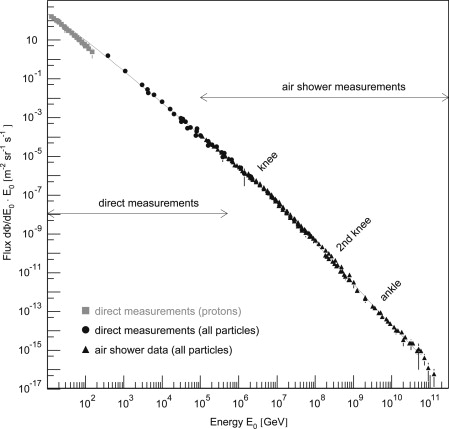
\includegraphics[width=.55\textwidth]{figs1/CRspectrum}
	\caption{\label{fig:CR}All-particle energy spectrum of CRs as measured directly with detectors above the atmosphere and with air shower detectors. Figure taken from \cite{energy_spec}.}
\end{figure}

The features of the CR spectrum are probably indications of the different source populations in energy range and location. Below the knee, sources are believed to be of galactic origin. Above the ankle, the decrease is possibly due to the CR sources reaching their maximum possible energy or to the fact that CRs are able to escape from the galactic magnetic field. In contrast, CRs above the ankle are believed to correspond to populations of extragalactic sources, since the astrophysical objects in the galaxy do not meet the necessary requirements to accelerate them at such energies.

\subsection{CR--$\boldsymbol{\gamma}$--$\boldsymbol{\nu}$ relation}
\label{sec:CR-gamma}

%As mentioned, there are clues that CRs and $\gamma$-radiation are produced by the same astrophysical sources. The connection between these two kinds of radiation and the production of

The connection between CRs and $\gamma$-radiation with the production of cosmic neutrinos is basically due to the interactions of CRs with the environment where they are produced. Since CRs are mainly accelerated protons, their interactions can be reduced to two types:

\begin{enumerate}[label=\textbullet]
	
    \item $\boldsymbol{p\,\gamma}$ \textbf{processes}. The most significant one is the Delta resonance:
	
	$$
	p\,\gamma \rightarrow \Delta^+ \left\{\begin{aligned}
	& \xrightarrow{\text{2/3}} p\,\pi^0 \\
	& \xrightarrow{\text{1/3}} n\,\pi^+ 
	\end{aligned}\right.
	$$
	
	This process is particularly interesting in the case of the interaction of CRs with the CMB, the GZK effect, which is expected to significantly reduce the CR flux above $\sim$100 EeV and produce diffuse fluxes of $\gamma$-rays and neutrinos. Thus, a neutrino detected with an energy above that cutoff limit has certainly a cosmic origin, since it cannot be produced by CRs in the atmosphere, which is the major background contribution in the detectors (see \autoref{subsec:background}).
	
	\item $\boldsymbol{p\,p}$ \textbf{processes}. If the matter density of the environment is larger than that of the radiation, CR interactions are dominated by $p\,p$ processes,  the most frequent being:
	
	$$
	\begin{aligned}
	p\,p \rightarrow p\,p\,\pi^0 \quad &\quad p\,p \rightarrow p\,n\,\pi^+ \\
	p\,n \rightarrow p\,n\,\pi^0 \quad &\quad p\,n \rightarrow p\,p\,\pi^-
	\end{aligned}
	$$
\end{enumerate}

These are hadronic processes, but they can produce leptons through pions that frequently decay into photons and leptons:

$$
\setlength{\jot}{2pt}
\begin{aligned}
\pi^0 \rightarrow & \,\gamma\,\gamma \\[15pt] % <— extra vertical space here
\pi^+ \rightarrow & \,\mu^+ \, \nu_\mu \\
& \hookrightarrow e^+ \, \nu_e \, \bar{\nu}_\mu
\end{aligned}
\qquad\qquad
\begin{aligned}
\pi^- \rightarrow & \,\mu^- \, \bar{\nu}_\mu \\
& \hookrightarrow e^- \, \bar{\nu}_e \, \nu_\mu
\end{aligned}
$$

Thus, the decay of pions from CRs are related to $\gamma$-ray and neutrino production. The ratio $\gamma/\nu$ depends on the rate of $p\,p$ and $p\,\gamma$ processes. Therefore, astrophysical studies based on photons and neutrinos are complementary and necessary to understand the underlying physics of astronomical objects.

\section{Cosmic neutrino sources}

Cosmic neutrinos can be produced in a wide variety of astrophysical objects and through several mechanisms and exotic processes \cite{Agus, sources, sources2, sources3}. The sources can be divided in two categories: galactic and extragalactic sources.

\subsection{Galactic}

\begin{enumerate}[label=\textbullet]

	\item Shell-type Supernova Remnants (SNRs): In a supernova most of the star material is ejected at velocities up to $10\%$ the speed of light. The shock waves generated against the interstellar medium creates the proper conditions to induce particle acceleration. Interaction of these CRs with previously expelled star material and interstellar medium would give rise to neutrino and gamma-ray fluxes.
	
	\item Pulsar Wind Nebulae (PWNe) or pleirons: It refers to a particular kind of SNRs where the supernova left a neutron star or pulsar as remnant. This compact object, with a strong magnetic field and a fast rotation, induces a continuous particle acceleration that flows out in jets.
	
	\item X-Ray Binaries (XRBs): Binary star systems where one of the components is a collapsed object such as a white dwarf, a neutron star or a black hole. The companion star fuels material into the compact partner forming an accretion disk around it. On this accretion process, falling material reach temperatures high enough to emit X-rays.
	
	\item Galactic centre: The centre of the Milky Way hosts a supermassive black hole (Sagittarius A*) surrounded by multiple SNRs, PWNe and XRBs as well as other TeV $\gamma$-ray sources. Neutrino emission seems likely since meson decay is the only feasible mechanism able to diffuse $\gamma$-ray emission in this region.
	
\end{enumerate}

\subsection{Extragalactic}

\begin{enumerate}[label=\textbullet]

	\item Gamma-Ray Bursts (GRBs): Short-lived flashes with the highest known peak luminosities, being the the most energetic events ever detected. They are linked with asymmetric supernovas whose jets point towards the Earth and with compact objects merging. As transitional short events, their time information allows to put strong constrains on predictions.
    
	\item Active Galactic Nuclei (AGNs): In terms of time-integrated energy output and sustained luminosity, their energy release far exceeds that of any other known population, such as SNRs or GRBs. Roughly 1\% of all bright galaxies possess an active nucleus in which the equivalent of the radiation power of more than the combination of all stars in our galaxy is radiated from a region smaller than the size of the solar system. The brightest AGNs on $\gamma$-ray emission are called \textit{blazars}. These objects are expected to be AGNs with active relativistic jets pointing towards the Earth. The object PKS 0735+17 is a particular case of these objects, which will be the first use case for the method developed in \autoref{chap:ml}. 
	
	\item Starburst galaxies: These galaxies host regions with a very high star formation rate compared to regular galaxies. As a consequence, supernovas take place frequently enough to expect an important CR production.
	
	\item Galaxy clusters: They are the largest gravitationally bounded objects in the universe. Their possible neutrino production is expected from $p\,p$ interactions between CRs and intracluster material.
	
	\item Cosmogenic (GZK) neutrinos: A diffuse neutrino flux is expected to be produced as a consequence of the GZK effect through the Delta resonance when CRs have enough energy.
\end{enumerate}

\section{Detection principle}

The properties that make neutrinos good candidates as astronomical messengers also make them very hard to detect. The first proposal to detect cosmic neutrinos was described by M. A. Markov in 1960 \cite{astro_neutrino}. In order to discriminate the incoming direction, neutrinos have to be detected indirectly through their interactions with matter at the Earth. The proposal was to detect charged secondary particles from the neutrino-nucleon interaction, such as muons, via emission of Cherenkov light \cite{Cheren}. The detector, a three-dimensional array of photomultiplier tubes (PMTs) inside a transparent medium like water or ice, collects the Cherenkov radiation induced by the passage of the relativistic charged particles inside or near the instrumented volume. Due to the low cross section of the neutrino-nucleon interaction, the volume of detection is needed to be very large --at the order of 1000 m$^3$--, so it was proposed to set the detectors deep in the ocean or in an underground lake. The information registered by the PMTs is used to infer the arrival direction of the parent neutrino and an estimation of its energy. Thus, the basic idea of a neutrino telescope was born.

A problem with this detection mechanism is that charged particles produced by other mechanisms are also detected. Huge amounts of muons are produced by CRs colliding with the atmosphere. Therefore, neutrino telescopes are optimised to detect the light from up-going particles produced by neutrinos which have traversed the Earth. Hence, the detection of down-going atmospheric muons, which is the major background contribution, is heavily reduced. Nevertheless, contributions to the background events occur due to the production of atmospheric neutrinos and bioluminescence. These topics are discussed in detail in the following sections.

\subsection{Neutrino interactions with matter}

Neutrinos only interact through the weak force. There exists two possible channels of interaction with matter (typically with a nucleus, $N$) \cite{neutrino_interactions}: 

\begin{enumerate}[label=\textbullet]
	\item Charged Current (CC): The interaction is produced through the $W^{\pm}$ boson.
    
	$$
    \nu_l \, N  \rightarrow  \,l^- +\mathrm{hadronic~jet} \qquad \qquad \bar{\nu}_l \, N  \rightarrow  \,l^+ +\mathrm{hadronic~jet}
    $$
    
    \hide{
    $$
    \setlength{\jot}{2pt}
	\begin{aligned}
	\nu_l \, N  \rightarrow & \,l^- +\mathrm{hadronic~jet} \\
	\bar{\nu}_l \, N  \rightarrow & \,l^+ +\mathrm{hadronic~jet}
	\end{aligned}
	$$
    }
	
	\item Neutral Current (NC): The interaction is produced through the $Z^0$ boson.
	
    $$
	\nu \, N  \rightarrow \nu \, N
	$$
	
\end{enumerate}

Depending on the type of interaction and the lepton flavour, two types of event signatures can be detected in a neutrino telescope \cite{inter}. Track-like events are originated from CC of muon-(anti)neutrino interactions ($\nu_\mu^{CC}$). The muon produced can travel very long distances before decaying. Thus, this kind of events are well suited for direction reconstructions. The angular difference between the primary neutrino and the muon is usually $<1^\circ$ for neutrino energies around 1 TeV, with finer alignments as the energy increases.

The second type of signatures are cascades, also known as shower-like events. These are produced by all NC interactions and by electronic CC ($\nu_l^{NC}$, $\nu_e^{CC}$). In the NC interactions, the energy transferred to the nucleus produce a hadronic shower, while a residual part of the energy is carried by a secondary neutrino. In the electronic CC, the produced electron rapidly loses energy via \textit{bremsstrahlung} and pair production, generating an electromagnetic shower and depositing almost all the energy near the interaction vertex. Since cascades do not spread much, direction reconstruction of shower events is typically more difficult than that of track events, whereas for the energy reconstruction, the trend is the opposite.

The $\nu_\tau^{CC}$ interactions are usually treated separately, since they can produce both shower and track events, depending on the energy of primary neutrinos and the nature of the secondary interaction. In contrast to muons, tauons have a much shorter lifetime, so they travel only from metres to kilometres, depending of their energy, before decaying. If the tauon decays into a muon, the resulting particle can produce a long track, being indistinguishable from a $\nu_\mu^{CC}$ interaction by the detector. If the tauon produces an electron or a tau-neutrino, the result is an electromagnetic or hadronic shower, respectively, generating a ``double bang'' signature, which refers to the sequence of two consecutive cascades. \autoref{fig:inter} shows schematic views of the most relevant processes.

\begin{figure}[htbp]
	\centering
	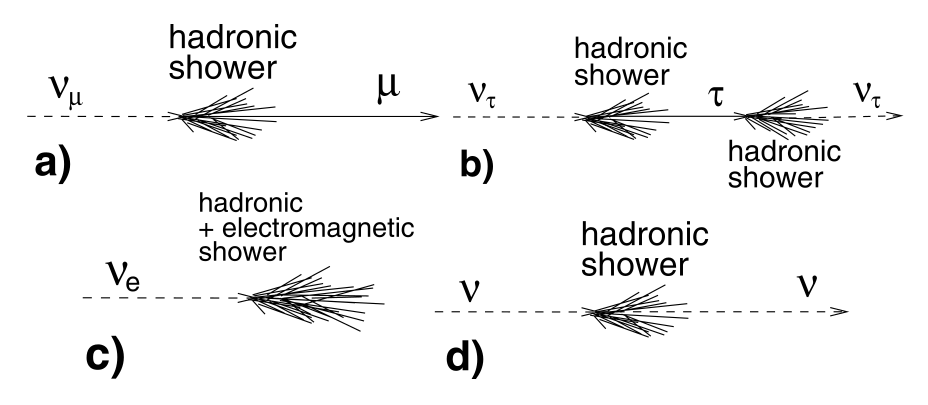
\includegraphics[width=.6\textwidth]{figs1/CC_NC}
	\caption{\label{fig:inter}Schematic view of the most relevant event signatures in a neutrino telescope: $\nu_\mu^{CC}$ (a), $\nu_\tau^{CC}$ double bang (b), $\nu_e^{CC}$ (c) and all flavour $\nu^{NC}$ (d). Figure taken from \cite{image_inter}.}
\end{figure}


\subsection{Cherenkov radiation}

Cherenkov radiation is emitted by charged particles crossing a dielectric medium with speed exceeding that of light in the medium \cite{Cheren}. The charged particle polarizes the molecules along its trajectory, but only an overall dipole moment is present when the particle moves faster than light in the medium. Cherenkov light is emitted when the electrons of the dielectric medium restore themselves to equilibrium after the disruption has passed, creating a coherent radiation emitted in a cone with a characteristic angle $\theta_C$:

\begin{equation}
\cos(\theta_C)  = \frac{1}{\beta \, n},
\end{equation}

where $\beta = v/c$ is the particle velocity in units of $c$ and $n$ is the medium refractive index. 

The emission spectrum is continuum and its intensity increases with the frequency up to blue and ultraviolet (UV) wavelengths, above which, the emission is no longer possible. The amount of Cherenkov photons ($N_\gamma$) emitted by a particle of charge Z per unit wavelength interval (d$\lambda$) and unit distance traveled (d$x$) is \cite{N_cheren}:

\begin{equation}
\frac{\mathrm{d}N_\gamma}{\mathrm{d}\lambda \mathrm{d}x} = \frac{2\pi\alpha Z^2}{\lambda^2}\left( 1-\cos^2(\theta_C) \right),
\end{equation}

where $\alpha$ is the fine structure constant.

\subsection{Background noise} % contamination? events?
\label{subsec:background}

There are challenges using Cherenkov light of secondary particles as detection principle. First, other processes in the atmosphere produce charged particles that are detected by neutrino telescopes. CR showers in the atmosphere produce a continuous isotropic flux of neutrinos. They are called atmospheric neutrinos and are the biggest source of noise when trying to detect cosmic neutrinos. Except for ultra-high energy events, this contribution to the background noise impedes event to event detection. Detections are then based on statistical analysis.

Second, CR showers in the atmosphere produce atmospheric muons. Since the telescopes only detect charged particles, they leave the same signature as a secondary particle from a neutrino interaction. To diminish the amount of atmospheric muons being detected as neutrino muons, neutrino telescopes usually point downwards, using the Earth as a shield. This is because the probability of a muon traversing the Earth is null. However, upward reconstruction from a downwards particle, although unlikely, can happen.

Therefore, a good understanding and estimation of the background is capital in neutrino telescopes. It is needed to find evidences of a cosmic neutrino flux from event excesses, differences in spectrum energy or in arrival directions.% \nota{Tal vez ampliar un poco, ya veremos}


\section{Neutrino telescopes}

The first attempt of building a neutrino telescope was the DUMAND project \cite{Dumand} in the late 1970s. It aimed to deploy a detector in the Pacific Ocean, near to the island of Hawaii. The project was cancelled due to technical and financial problems, but it set the basis for the following neutrino telescopes. The relay of the high-energy neutrino astronomy was taken by the Baikal telescope \cite{Baikal1}, located in the depths of the Russian Lake Baikal, and by the AMANDA telescope \cite{Amanda}, under the ice of the South Pole. The experience of the DUMAND project was taken up by ANTARES \cite{Antares}, leading afterwards to the, already under construction, largest deep-sea neutrino telescope, KM3NeT \cite{km3net}. The Italian NEMO \cite{NEMO} and the Greek NESTOR \cite{NESTOR} initiatives, although never completed, also contributed to the development that eventually converged in KM3NeT. In parallel, there is also a new project, called P-ONE, still in the research and development stage \cite{Pone}, and initiatives in China in the same direction, such as TRIDENT \cite{TRIDENT}. Here, we briefly detail the three currently active detectors.

%The first attempt of building a neutrino telescope was the DUMAND project \cite{Dumand} in the late 1970s. It aimed to deploy a detector in the Pacific ocean, near to the island of Hawaii. The project was cancelled due to technical and financial problems, but it set the basis for the following neutrino telescopes. The relay of the high-energy neutrino astronomy was taken by the Baikal telescope \cite{Baikal1}, located in the depths of the Russian Lake Baikal, and by the AMANDA telescope \cite{Amanda}, under the ice of the South Pole. The experience of the DUMAND project was taken up by ANTARES\cite{Antares}, leading afterwards to the, already under construction, largest deep-sea neutrino telescope, KM3NeT \cite{km3net}. There is also a new project, called P-ONE, still in the research and development stage \cite{Pone}. The ANTARES telescope will be detailed in \autoref{chap:antares}. In the following paragraphs, the three currently active detectors will be briefly detailed.

\subsubsection*{Baikal-GVD}

The Baikal neutrino detector, first deployed in 1993, underwent a significant upgrade to become the Baikal Gigaton Volume Detector (Baikal-GVD) \cite{Baikal}. Since its inception, the sensitivity and coverage of the experiment have progressively improved. Currently, the facility incorporates 2304 MPTs deployed at depths reaching up to 1366 meters. The detector’s infrastructure consists of vertical strings anchored to the lakebed and stabilized by buoyant systems at their upper ends. Each string has 36 optical modules (OMs), with every module equipped with a 10-inch, high-quantum-efficiency PMT oriented downward to optimize detection capabilities.

\subsubsection*{IceCube}

The IceCube Neutrino Observatory, constructed between 2005 and 2010, is the successor to the AMANDA (Antarctic Muon and Neutrino Detector Array) experiment located in the South Pole’s glacial ice \cite{IceCube}. Its detector encompasses a cubic kilometre of pristine Antarctic ice, optimized for high transparency. The infrastructure comprises 86 vertical strings positioned above the bedrock at depths of 1.5 to 2.5 kilometres. These strings, spaced 125 meters apart in a grid of equilateral triangles, hold 5,160 Digital Optical Modules (DOMs). Each DOM features a spherical, pressure-resistant housing containing a 25-centimetre PMT and digitization electronics. Modules are spaced 17 meters vertically along each string. To improve sensitivity to low-energy neutrinos, a dense central sub-array named DeepCore employs high-quantum-efficiency PMTs. The observatory also integrates IceTop, a surface-level cosmic ray detector, forming a comprehensive detection system. Full operational data collection began in May 2011. In 2014, IceCube achieved a milestone by confirming the first astrophysical neutrinos of cosmic origin \cite{ice}. Since then, IceCube has measured a diffuse flux of high-energy astrophysical neutrinos and provided important constraints on their energy spectrum. The collaboration has also reported high-profile detections of neutrinos coincident with blazar flares, contributing to the identification of potential cosmic neutrino sources \cite{iceblazar, icediffuse}.


\subsubsection*{KM3NeT}

The Cubic Kilometre Neutrino Telescope (KM3NeT) is still under construction, but already taking data since 2019. It is a deep-sea neutrino telescope in the Mediterranean Sea and, once completed, it will be the largest neutrino telescope in the world. It is composed of two separate detectors: ARCA and ORCA (Astroparticle/Oscillation Research with Cosmics in the Abyss) \cite{km3net1}.

ARCA’s primary scientific objective is to identify high-energy neutrinos originating from cosmic sources. Specifically, the experiment focuses on investigating potential cosmic ray accelerators within the Milky Way to detect neutrino emissions associated with these astrophysical phenomena. Located approximately 100 kilometres off-shore Portopalo di Capo Passero (Italy), the infrastructure operates at a depth of about 3,500 metres. The finalized design includes two independent blocks, each composed of 115 Detection Units (DUs), collectively instrumenting a volume of roughly one cubic kilometre. Each DU extends vertically for approximately 700 meters, with 18 DOMs distributed at 36-meter intervals starting 80 meters above the seabed. The horizontal separation between adjacent detection strings is approximately 95 metres. At the time of writing this thesis (October~2025), it is composed of 51 DUs. Remarkably, ARCA was able to detect in February 2023 --when only 21 DUs were working-- a neutrino with the highest energy ever recorded \cite{nature}.

ORCA is optimized for less energetic neutrinos, in the range of a few hundreds GeV, in order to study oscillations and mass ordering, among other exotic physics. Located about 40 kilometres off-shore Toulon (France), at a depth of 2,450 metres. When complete, it will be composed of only one building block with 115 DUs, each DU holding 18 DOMs spaced 9 metres apart in the vertical direction. The horizontal spacing between each DU string will be of around 20 metres. ORCA has then a smaller, but more densely instrumented volume compared to ARCA, better aligned to focus in a lower energy range. At the time of writing this thesis (October~2025), ORCA is composed of 24 DUs.



% -------------------------------------------------------
\part{New reconstruction method for ANTARES single-line events based on Machine Learning: \emph{N}-fit}
\label{part:2}

\chapter[Machine Learning introduction and \emph{N}-fit method development]{Machine Learning introduction and \emph{N}-fit method development}
\label{chap:ml}

%\nota{Comprobar todas las referecnias, meter plots faltantes que en el paper están en el apéndice (siguiente capítulo), comprobar que la escritura tenga sentido (más bien cuando todo acabe) y cambiar el título del capítulo.}


%The $N$-fit reconstruction algorithm is the end product of training a set of supervised deep neural networks (DNNs). In this chapter, we first introduce the Deep Learning tools employed in its configuration along with the innovative use we make of them. Then, we present how we preprocess the input data to the algorithm. Finally, we explain specific details in the development of the $N$-fit algorithm related to results.

The $N$-fit reconstruction algorithm is motivated by a longstanding limitation in ANTARES: for \emph{single-line} (SL) events --typically produced at lower energies-- the standard reconstruction does not provide an azimuthal estimation, leaving the event direction partially unconstrained. Although SL events provide a poorer geometrical baseline than multi-line tracks, they constitute a sizeable fraction of the data at low energy and can be valuable for several physics analyses (e.g., oscillation studies and solar dark-matter searches). Improving their directional reconstruction --particularly recovering azimuthal information-- directly increases the usable statistics and the scientific reach of the detector.

$N$-fit addresses this by training a set of supervised Deep Learning (DL) models tailored to SL topology, aiming to infer direction, event geometry, energy, and class with associated uncertainties. In this chapter, we first introduce the DL tools employed in its design together with the specific, innovative ways we apply them. We then describe the preprocessing pipeline that maps ANTARES data to network inputs. Finally, we detail the development choices behind $N$-fit and present the resulting performance, highlighting the impact on analyses that rely on low-energy SL events.


\section{Deep Learning built-in blocks}
\label{sec:N-fit}

The key feature for the successful performance of the $N$-fit algorithm is the integration of several Deep Learning tools. In this section, we unravel the algorithm: first, we introduce the very basics of artificial neural networks, on which the algorithm is based; then, we describe deep convolutional networks (DCNs) and mixture density networks (MDNs), which play an essential role in $N$-fit's capabilities. Lastly, we describe how we utilized different aspects of transfer learning (TL) to enhance challenging reconstruction analyses, such as energy estimation and event classification.

\subsection{Basics of Artificial Neural Networks}
\label{subsec:ANNs}

Neurons are the core units of neural network models. The basic neuron model in artificial neural networks is the perceptron \cite{perceptron}, which is inspired by the non-linear transduction of synaptic input summation in biological neurons towards action potential firing. Mathematically, the output ($y$) is described as the result of a nonlinear \textit{activation} function of a weighted linear combination of synaptic inputs:

\begin{equation}
	\label{eq:perceptron}
	y = f\left( \sum_i w_i \cdot x_i + b \right) =  f\left( \vec{w}\cdot\vec{x} +b \right),
\end{equation}

where $\vec{x}$, $\vec{w}$, and $b$ represent inputs, weights, and the neuron's bias, respectively. Even though this represents a strong oversimplification of the nonlinear dynamics of biological neurons in the brain, such a computation is capable of mapping arbitrary input-output functions efficiently if multiple perceptrons are present in layers, creating a \textit{feed-forward} network (\autoref{fig:feed-forw}). In $N$-fit, the Rectified Linear Unit \cite{relu} --defined as $\mathrm{ReLU}(x)=\max\{0,x\}$-- is used as the activation function of neurons in the hidden layers.

\begin{figure}[htbp]
	\centering
	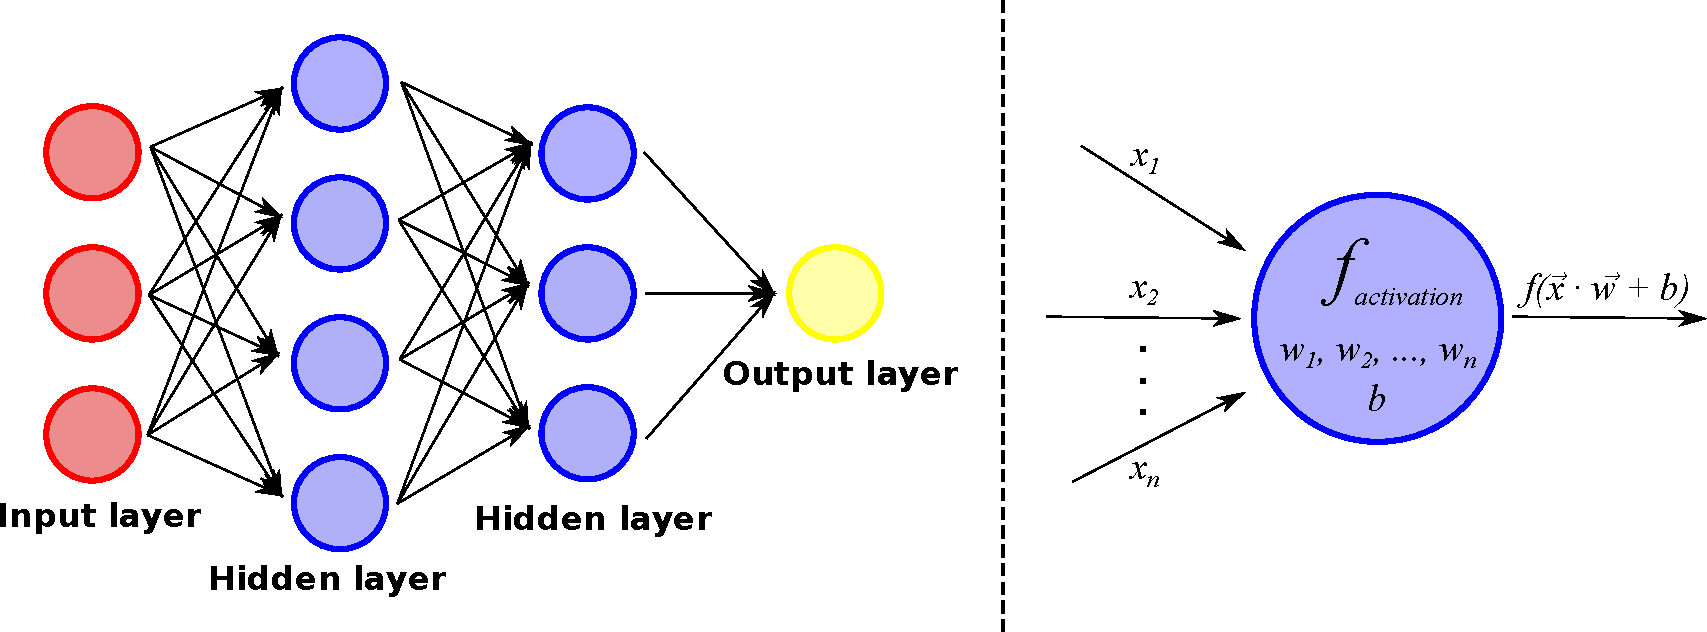
\includegraphics[width=.95\textwidth]{figs2/feed_forward.pdf}
	\caption{\label{fig:feed-forw}Schematic diagram of a simple feed-forward neural network. Circles represent neurons, and arrows represent synaptic connections. In general, more than a single output can be considered.}
\end{figure}


%The final architecture developed for both track and shower events is shown in Figure \ref{fig:network}. The weights initialization was done following Glorot et al. proposal \cite{Glorot} for convolutional layers and He et al. proposal \cite{He} for feed-forward (or dense) layers. To diminish over-fitting during training, we used early stopping \cite{EarlyStop} with a \textit{patience} of 10 epochs, for a maximum of 150. In each epoch, learning batches of 64 input elements were considered. We used the Adam algorithm \cite{Adam} as the learning optimizer because it is able to dynamically regulate the learning rate, which was initialized at $0.001$.


Each layer in the network model processes a level of internal representation that transmits information from one layer to the next. One of the main characteristics of deep vs. shallow learning is precisely its power of abstraction, which is achieved by significantly increasing the number of layers. Data fixes the number of neurons in the input, whereas the number of outputs is concomitant to the question that the model is designed to address. In contrast, the number of hidden layers and the number of neurons in them can vary. These are examples of hyper-parameters that need to be explored while testing the network's performance. Similarly, the learning process is also sensitive to the network's initialization \cite{ini_weights}. We initialized weights and biases randomly following the proposal of He et al. \cite{He} for all the feed-forward layers in the $N$-fit algorithm.

During training in supervised machine learning, the loss function computes the error committed between the network's output and the desired output in data batches (of 64 events in $N$-fit). Weights and biases are updated following error backpropagation, which uses gradient descent to propagate the output loss backwards through the network from the output layer, through the hidden layers, to the input layer. While there are several optimization algorithms based on error backpropagation \cite{SGD}, $N$-fit uses the Adam algorithm \cite{Adam} because it dynamically self-regulates the learning rate, which controls the pace at which learnable parameters in the network adapt. The learning rate was initialized at $0.001$ in every $N$-fit training process.

Typically, the learning procedure iterates over multiple epochs until a predetermined number of cycles is completed, where an epoch constitutes one complete pass of the entire training dataset through the neural network. However, an optimization strategy called Early Stopping enables premature termination of training before reaching this preset epoch threshold in order to diminish the risk of over-fitting \cite{EarlyStop}. This method monitors the loss of the validation dataset after each epoch and halts the process when two conditions are met: the validation loss reaches a minimum value, and a specified number of subsequent epochs (termed the \textit{patience} parameter) elapse without further reduction in validation loss. Upon stopping, the algorithm automatically restores the model parameters corresponding to the optimal validation performance observed during training. We set the maximum number of epochs to 150 and the patience to 10 epochs.

Another technique employed in order to avoid over-fitting is called DropOut \cite{Dropout}. It consists of randomly switching off a preset percentage of random neurons within a layer, so that the active neurons vary in each batch. In this way, DropOut prevents the neurons from becoming too specialised. In the $N$-fit algorithm, 20\% of the neurons from the convolutional block outputs were randomly dropped (i.e. their activation was set to 0) before feeding the first feed-forward layer.


\subsection{Deep Convolutional Networks}
\label{subsec:DCN}

Convolutional neural networks (CCNs) are a class of neural network models designed for processing structured grid data, such as images and image-like tensors \cite{CNN}. Inspired by the human visual system, they are built to recognize patterns and spatial hierarchies efficiently. Unlike traditional fully connected neural networks such as feed-forward ones, which treat every input as independent, CNNs leverage local connectivity, weight sharing, and hierarchical feature extraction to reduce the computational complexity while enhancing learning efficiency. At the heart of a CNN are convolutional layers, which are composed of small, trainable filters that slide over the input image to extract meaningful patterns.  These filters evolve over time through training, adapting to detect increasingly sophisticated features in deeper layers. Initially, filters may identify simple edges or gradients, but as they propagate through deeper layers, they start recognizing textures and shapes. The weight updates are governed by backpropagation and gradient descent, ensuring that the filters become more attuned to distinguishing relevant features from noise. After convolutional operations, the activation function introduces non-linearity to the network. In $N$-fit convolutional layers, ReLU is used, as well as in the fully connected layers. Without the activation function, CNNs would merely perform linear transformations, limiting their ability to capture complex representations.

Pooling layers follow the convolutional layers to refine the feature maps by reducing their spatial dimensions. These layers do not have trainable weights but instead apply fixed operations such as max pooling or average pooling. We used max pooling, the most common method, that retains the most prominent feature in a given region, preserving the strongest activations while discarding less relevant information. This downsampling process helps mitigate overfitting by reducing the number of parameters, thereby improving generalization. By compressing the feature maps, pooling layers also allow subsequent convolutional layers to focus on more abstract features without excessive computational overhead.

Deep Convolutional Networks (DCNs), meaning Deep CNNs, are the main tools used in the development of $N$-fit. DCNs extend traditional CNNs by stacking multiple convolutional, activation, and pooling layers to extract increasingly abstract and hierarchical features from input data. We processed ANTARES data generating image-like tensors that serve as inputs (see \autoref{sec:data}). Weights initialization followed Glorot et al. proposal \cite{Glorot} for every convolutional layer in $N$-fit. 

While basic CNNs can capture low-level patterns such as edges and textures, DCNs leverage deeper architectures to detect complex structures, object parts and entire objects with high accuracy. As the depth increases, feature maps transition from simple to highly abstract representations, enabling superior generalization and performance in tasks like image recognition and object detection. Training DCNs introduces challenges such as vanishing gradients and computational inefficiency. They are addressed through techniques like batch normalization, which we considered in $N$-fit. By deepening the network, DCNs significantly enhance the ability to learn intricate patterns, making them the backbone of state-of-the-art deep learning applications. Lastly, the extracted features from the convolutional layers are fed into fully connected layers, such as those in the feed-forward network explained earlier. At this stage, the network shifts from learning spatial hierarchies to making final predictions. 

\subsection{Mixture Density Networks}
\label{subsec:MDN}

Mixture Density Networks (MDNs) extend traditional regression neural networks by predicting complex, multimodal probability distributions instead of deterministic single-point estimates \cite{MDN}, making them ideal for estimating uncertainty in data. A measure of uncertainty is essential for selecting the most reliable estimates in posterior physics analyses.

The outputs of a MDN model represent the necessary parameters to create the multimodal probability density function from Gaussian kernels. Thus, instead of the typical output $\vec{y}_{p}$ for a single multidimensional prediction, the outputs of the network consist of means $\vec{\mu}_i$, variances $\sigma_i$ and mixture weights $\alpha_i$ (assuming that the outputs are statistically independent):

\begin{equation}
	PDF(\vec{y}_p) = \sum_i^n \alpha_i \cdot N(\vec{\mu}_i, \sigma_i; \vec{y}_p), \quad \quad \text{such that} \quad \sum_i^n \alpha_i = 1,
\end{equation}

where $N(\vec{\mu}, \sigma;\, \vec{y}_p)$ is a multi-dimensional isotropic Gaussian function. The number of Gaussian distributions $n$ must be hand fixed and predicted variances must always be positive, using the appropriate activation function --$N$-fit uses $\text{ELU}+1$ (ELU being the Exponential Linear Unit function). Similarly, the mixture weights use a softmax function to ensure they add to one. The network model learns to predict the parameters of these Gaussians --means, variances, and mixture weights-- using a specialized loss function based on maximum likelihood estimation (MLE), where the network is optimized to maximize the probability of the observed data under the predicted mixture model (\ref{eq:logloss}):

\begin{equation}
	\label{eq:logloss}
	\mathcal{L} = -\ln \left\{ \sum_i^n  \frac{\alpha_i}{(2\pi)^{c/2}\sigma_i^c}\exp\left( -\frac{||\vec{y}_t-\vec{\mu}_i||^2}{2\sigma_i^2} \right) \right\},
\end{equation}

where $c$ is the dimension of the output vector $\vec{y}_t$. In the development of $N$-fit, we only needed to parametrise each of our reconstructed parameters, following each a single Gaussian mode. With $c=1$, the loss function is reduced to:% (\ref{eq:loglossfinal}):

\begin{equation}
	\label{eq:loglossfinal}
	\mathcal{L} = \ln(\sqrt{2\pi}\sigma) + \left( \frac{(y_t-\mu)^2}{2\sigma^2} \right).
\end{equation}

This is different from traditional loss functions like mean-squared error (MSE), as it allows the model to learn distributions that can accommodate multiple correct answers, such as in inverse problems, rather than forcing a single prediction. However, training MDNs can be challenging due to numerical instability, and difficulties in optimizing multiple parameters simultaneously. These effects can be mitigated using regularization techniques, careful initialization strategies, and robust optimization methods like Adam's. In addition to careful initialization and Adam's optimization, $N$-fit avoided numerical instability issues by adding a small contribution to $\sigma$'s activation function: $\text{ELU}+1+\epsilon$. The value $\epsilon = 10^{-5}$ was selected after a quick exploration, in which a balance was achieved between being small enough not to alter the results, but large enough to avoid instability.

By integrating neural networks with probabilistic mixture models, MDNs bridge the gap between deep learning and statistical modelling.

\subsection{Transfer Learning}
\label{subsec:TL}

Transfer learning (TL) refers to the technique of leveraging knowledge gained from previously trained neural network models to improve performance on related tasks \cite{Transfer}. In the context of $N$-fit, we adopt two distinct paradigms of TL: \emph{direct transfer learning}, based on model reuse through layer freezing, and \emph{indirect transfer learning}, relying on knowledge distillation via dimensionality reduction.

% \paragraph{Direct Transfer Learning}

In direct TL, convolutional blocks from pretrained models are reused as fixed feature extractors in subsequent models. Specifically, networks trained for spatial reconstruction are repurposed for classification in $N$-fit between track and shower neutrino events by freezing their convolutional layers. These frozen components are connected in parallel to a feed-forward neural network (FFN), effectively enriching the classifier's input space with spatially encoded representations without requiring retraining of the feature extractors. This strategy benefits from the spatial specialization of each pretrained model and mitigates overfitting by reducing the number of trainable parameters for classification.

% \paragraph{Indirect Transfer Learning via PCA-based Knowledge Distillation}

Indirect TL in $N$-fit is achieved through knowledge distillation \cite{moslemi2024} from pretrained networks by extracting internal activations and transforming them into compact, informative representations using dimensionality reduction techniques. Specifically, this is accomplished using Principal Component Analysis (PCA), a linear dimensionality reduction technique that identifies orthogonal directions (principal components) along which data variability is maximized \cite{PCA}.

PCA is applied to neuron activations from the hidden layers of the networks trained for spatial reconstruction in $N$-fit, which are assumed to encode latent features relevant for energy estimation. These activations form a high-dimensional feature space, potentially redundant or noisy. With the PCA, we can reduce this space by projecting the original activations onto a lower-dimensional subspace defined by the principal components. Components are ordered by their explained variance, and only those contributing significantly to the total variance are retained. This selection ensures that the most informative and least correlated features are preserved.

The resulting low-dimensional vectors serve as inputs to a downstream FFN tasked with energy regression. This setup effectively transfers high-level abstract knowledge learned during direction and distance reconstruction, enabling the energy model to exploit interdependencies among event features not explicitly provided by the original inputs. More generally, this PCA-based approach enables a form of model-agnostic knowledge transfer, where the distilled representations serve as a bridge between pretrained networks and the target model.

Specific details on how Transfer Learning is applied to every reconstruction task are left to \autoref{sec:workflow}.

\section{Dataset preprocessing}
\label{sec:data}

The first step to apply $N$-fit to SL neutrino events was to preprocess the available data as image-like tensors. In this view, the ANTARES telescope is akin to a camera collecting 3D images at each time step, having as many pixels as OMs. For SL events, we created coloured 2D images, with time in one dimension (x-axis) and the storey of the line in the other (y-axis). 
% Creo que esto ya está dicho de antes y rompe el flow.
% Hits refer to detections in OMs that exceeded a threshold. 
The time stamp for each event was relative to the reference hit representing such event, which is the hit that occurred first in time, selected by the $\chi^2$-fit strategy. Next, all hits recorded by the OMs on the line covering a time window of -200 ns to 600 ns relative to the reference hit are selected. Cleaning noisy or background hits is left to the networks themselves. Colours resulted from combining the information provided by the three evenly distributed OMs in each storey. In each pixel of the 2D image, we inserted RGB channels to be informative of the event reconstruction in the horizontal (XY) plane, helping to estimate the azimuthal angle ($\phi$). More specifically, we weighted the angle to which each OM points in XY ($\alpha$) by its recorded voltage amplitudes ($A$). Mathematically, the transformation is represented in equation \ref{eq:RGB}.

\begin{equation}
	\label{eq:RGB}
	(R;G;B) = \left\{
	\begin{aligned}
		A\cdot(1-\tfrac{\alpha}{2\pi/3};\tfrac{\alpha}{2\pi/3};0) ~~~~~~
		\quad\text{if}~~&\alpha \in \left[0, \tfrac{2\pi}{3}\right]
		\\
		A\cdot(0;2-\tfrac{\alpha}{2\pi/3};\tfrac{\alpha}{2\pi/3}-1)
		\quad\text{if}~~&\alpha \in \left[\tfrac{2\pi}{3}, \tfrac{4\pi}{3}\right]
		\\
		A\cdot(\tfrac{\alpha}{2\pi/3}-2;0;3-\tfrac{\alpha}{2\pi/3})
		\quad\text{if}~~&\alpha \in \left[\tfrac{4\pi}{3}, \tfrac{6\pi}{3}\right]
	\end{aligned}
	\right.
\end{equation}

From the discrete hits, we built a continuous signal representing the hit amplitudes over time by applying a Gaussian kernel smoothing with $\sigma = 5$ ns, and then discretized this signal at regular intervals of 5 ns for each individual colour: $\{R(t);G(t);B(t)\}$. Finally, we re-centred the image based on the floor of the reference hit (a representative example is shown in \autoref{fig:RGB}).

Given the huge amount of data available from the ANTARES collaboration, we processed a subset ($\sim$10\%) of MC runs whose identification numbers end in ``0'' in the 2008--2017 period, to keep a good balance between training time and performance. The collected images of SL events were separated into track-like ($\nu_\mu^{CC}$) and shower-like ($\nu_\mu^{NC}$, $\nu_e^{CC}$, $\nu_e^{NC}$) simulations datasets, in order to train specialized models for each event topology. Each dataset was then randomly split in three sub-sets: train (60\%), validation (20\%), and test (20\%). Before feeding images to the network, a Z-score normalization was separately applied to each set. For this, we computed the mean and standard deviation of the respective train sub-sets and applied the transformation to all sub-sets to control for distribution shifts. After the development phase, we also processed other events types, such as simulations of atmospheric muons, random noise background events and real ANATRES data, for control analyses.

\begin{figure}[htbp]
	\centering
	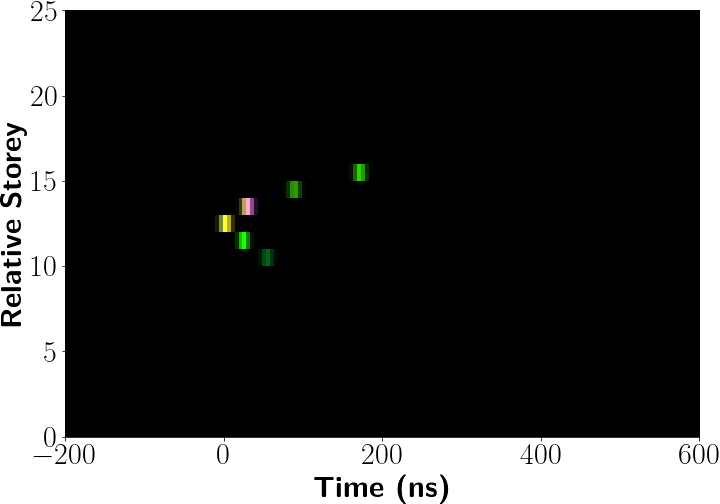
\includegraphics[width=.5\textwidth]{figs2/RGB.png}
	\caption{\label{fig:RGB}Normalized RGB image example of a track event.}
\end{figure}



%%%%%%%%%%%%%%%%%%%%%
%
%
%
%
%
%
%
%
%
%%%%%%%%%%%%%%%%%%%%%%

\section{\emph{N}-fit modular organization}
\label{sec:workflow}

The $N$-fit reconstruction strategy is subdivided into two branches specialized in each type of event: tracks and showers. Each branch cover the different aspects that fully describe neutrino events. The track-branch reconstructs the neutrino direction, the closest point of the secondary muon track to the detector line and the muon energy. Although the shower-branch also reconstructs the direction of the neutrino, it differs slightly in the other parameters, reconstructing the vertex point of the neutrino interaction and its energy. The two branches converge through TL in the classifier that divides the events in tracks or showers. Next subsections explain the details of these network models.

\subsection{Direction reconstruction}
\label{subsec:direction}

%The final architecture developed for both track and shower events is shown in Figure \ref{fig:network}. The weights initialization was done following Glorot et al. proposal \cite{Glorot} for convolutional layers and He et al. proposal \cite{He} for feed-forward (or dense) layers. To diminish over-fitting during training, we used early stopping \cite{EarlyStop} with a \textit{patience} of 10 epochs, for a maximum of 150. In each epoch, learning batches of 64 input elements were considered. We used the Adam algorithm \cite{Adam} as the learning optimizer because it is able to dynamically regulate the learning rate, which was initialized at $0.001$.

Several architectures of increasing complexity were analysed during the optimization of direction reconstruction models for track events. The key steps followed to measure and improve the model's performance are summarised below:

\begin{enumerate}[label={\textit{\roman*})}]
	\item Baseline Control Model: Feed-forward network of four hidden layers implemented to fully reconstruct the Cartesian components of the direction unit vector: $(X;Y;Z)$.
	
	\item Components Separation: Next, the model was divided to reconstruct $Z$ and $\{X,Y\}$ separately. Reconstructions were sequential, first $Z$, then $\{X,Y\}$. We regularized the value of the components $\{X,Y\}$ to penalize deviations of $(X;Y;Z)$ from unit vectors.
	
	\item MDNs and $\theta$ Representation: Point predictions were replaced by inferring probability distributions (MDN). The change did not vary performance but provided event uncertainty estimation, which is of major relevance as a quality metric in posterior physics analyses. Also, the network output $Z$ was replaced by the angle $\theta$, gaining a best estimation of the angle uncertainty, since no error propagation was needed to infer it. %resolution in the limit cases when $Z$ approaches one or minus one. \notaSA{esto último no se acaba de entender}
	
	\item Convolutional Layers: A significant improvement was observed by adding two convolutional layers before the dense network.
	
	\item Image Centring: Aligning events to a centred reference frame further enhanced performance, despite the architecture remained unaltered.
	
	\item Final Adjustments: The number of convolutional layers was optimized (see \autoref{tab:comparison}). From there on, additional layers provided only marginal changes in performance.
	
\end{enumerate}

The progression of the Mean Absolute Error (M.A.E.) through these steps is presented in \autoref{tab:comparison}. The final architecture is illustrated in \autoref{fig:network}. This optimized architecture for the track branch was then applied in the shower branch without further optimization.

% Yo creo que esto no hace falta:
% Additionally, an alternative approach was tested by computing the angle $\phi$ directly instead of $XY$, using techniques for periodic variables, an area where neural networks typically struggle. However, while the resolution remained similar, the reconstructed error did not behave properly. 

% \notaSA{yo añadiría dos filas más para las incertidumbres y allí donde no las contemple la red se  pone  --, así esa ya es de por si una mejora y permite comparar en los casos con los que sí que las contemplan, ya que cuanto menor sea su valor medio mejor, no?} \notaJGM{Lo de las incertidumbres me parece una buena idea, pero ahora mismo no dispongo de esos datos. En los informes originales yo no ponía esa información, de modo que tendrá que ver si tengo las redes entrenadas por ahí o re-entrenar para obtener esa info. Lo dejo como algo que se podría hacer, pero de momento para una primera revisión interna de ANTARES no creo que dé tiempo.}

\begin{table}[htbp]
	\centering
	\renewcommand{\arraystretch}{1.2} % Improves row spacing for better readability
	\begin{tabular}{|c|cc:cccc|}
		\hline
		\textbf{M.A.E.} & \textbf{\textit{i}} & \textbf{\textit{ii}} & \textbf{\textit{iii }} & \textbf{\textit{iv}} & \textbf{\textit{v}} & \textbf{\textit{vi}} \\ \hline
		$\boldsymbol{\theta}$ & $11.2^\circ$ & $10.5^\circ$ & $10.5^\circ$ & $9.6^\circ$ & $8.4^\circ$ & $7.4^\circ$  \\ %\hline
		$\boldsymbol{\phi}$ & $50.1^\circ$ & $49.5^\circ$ & $49.5^\circ$ & $46.2^\circ$ & $44.1^\circ$ & $41.4^\circ$ \\ \hline
	\end{tabular}
	\caption{\label{tab:comparison}Evolution of the Mean Absolute Error (M.A.E.) of the test data set along the key steps followed in the development and optimization of the $N$-fit algorithm for the direction reconstruction of tracks. $\sigma$ estimation was introduced in model (iii).}
\end{table}

\begin{figure}[htbp]
	\centering
	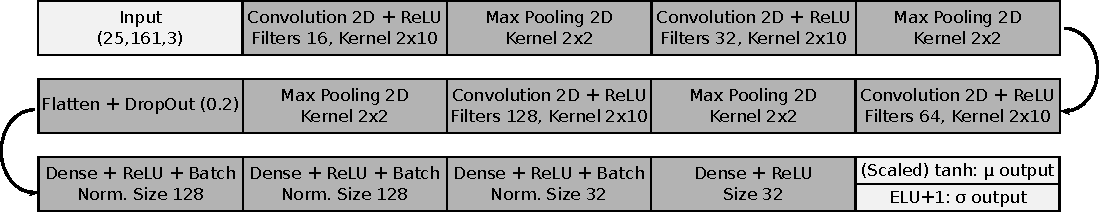
\includegraphics[scale=0.69]{figs2/DCN.pdf}
	\caption{\label{fig:network}Details of the direction neural network architecture. Note that for the $\theta$ prediction, we scaled the hyperbolic tangent activation function for $\mu_\theta$, so that its values lay in $[0, \pi]$ radians. No scaling was necessary for the prediction of $\phi$ since its estimation was derived from the Cartesian $\{X,Y\}$ components of the unit vector.}
\end{figure}

The loss function applied to the angle $\theta$ becomes eq. (\ref{eq:loss_theta}), where $\theta_t$ represents the true value of the angle $\theta$ for each neutrino event in the simulation.

\begin{equation}
	\label{eq:loss_theta}
	\mathcal{L} = \ln (\sqrt{2\pi}\sigma_{\theta}) + \frac{1}{2}\frac{(\theta_{t}-\mu_{\theta} )^2}{\sigma_{\theta}^2},
\end{equation}


A second network predicts the angle $\phi$ through its Cartesian coordinate values ($\mu_X$, $\mu_Y$) and their uncertainties ($\sigma_X$, $\sigma_Y$). The loss function was transformed consequently in equation (\ref{eq:loss_phi}):

%The other network must predict the $\phi$ angle. Since neural networks are inefficient at predicting periodic variables, we used the Cartesian coordinates $XY$ for the $\phi$ reconstruction, as well as their uncertainties. To this end, we used the following loss function:

\begin{equation}
	\label{eq:loss_phi}
	\begin{split}
		\mathcal{L} = &\ln (\sqrt{2\pi}\sigma_{X}) + \frac{1}{2}\frac{(X_{t}-\mu_{X} )^2}{\sigma_{X}^2}+\\
		+ &\ln (\sqrt{2\pi}\sigma_{Y}) + \frac{1}{2}\frac{(Y_{t}-\mu_{Y} )^2}{\sigma_{Y}^2}+\\
		+ &(1-[\mu_{X}^2+\mu_{Y}^2+\cos^2(\mu_{\theta})])^2.
	\end{split}
\end{equation}

The last term in equation (\ref{eq:loss_phi}) regularizes the output of the network, penalizing deviations of $(X;Y;Z)$ from unit vectors. %where the Z component is derived from the $\theta$ prediction as follows: $\mu_Z=\cos(\mu_\theta)$.
To infer the uncertainty of $\phi$, we performed a quadratic error propagation as shown in equation (\ref{eq:error_prop}).

\begin{equation}
	\label{eq:error_prop}
	\sigma_{\phi}^2 = \left(\frac{\partial \phi}{\partial \mu_X}\cdot \sigma_X\right)^2 + \left(\frac{\partial \phi}{\partial \mu_Y}\cdot \sigma_Y\right)^2 \Rightarrow
	\sigma_{\phi} = \frac{\sqrt{\sigma_X^2\cdot \mu_Y^2+\sigma_Y^2\cdot \mu_X^2}}{\mu_X^2+\mu_Y^2 }
\end{equation}

Note that the uncertainty estimation assumes a Gaussian distribution. This means that distribution of errors should become wider although centred with growing $\sigma$ values. For most of the range this is precisely the case when tested, especially for $\theta$ (\autoref{fig:sigma}). As for the uncertainty of the direction reconstruction ($\sigma_{\Omega}$),  we used the expression (\ref{eq:sigma_omega}) derived from the solid angle definition: 

\begin{equation}
	\label{eq:sigma_omega}
	\sigma_\Omega = \sqrt{\sin^2(\theta)\sigma_\phi^2 + \sigma_\theta^2}.
\end{equation}

\begin{figure}[htbp]
	\centering
	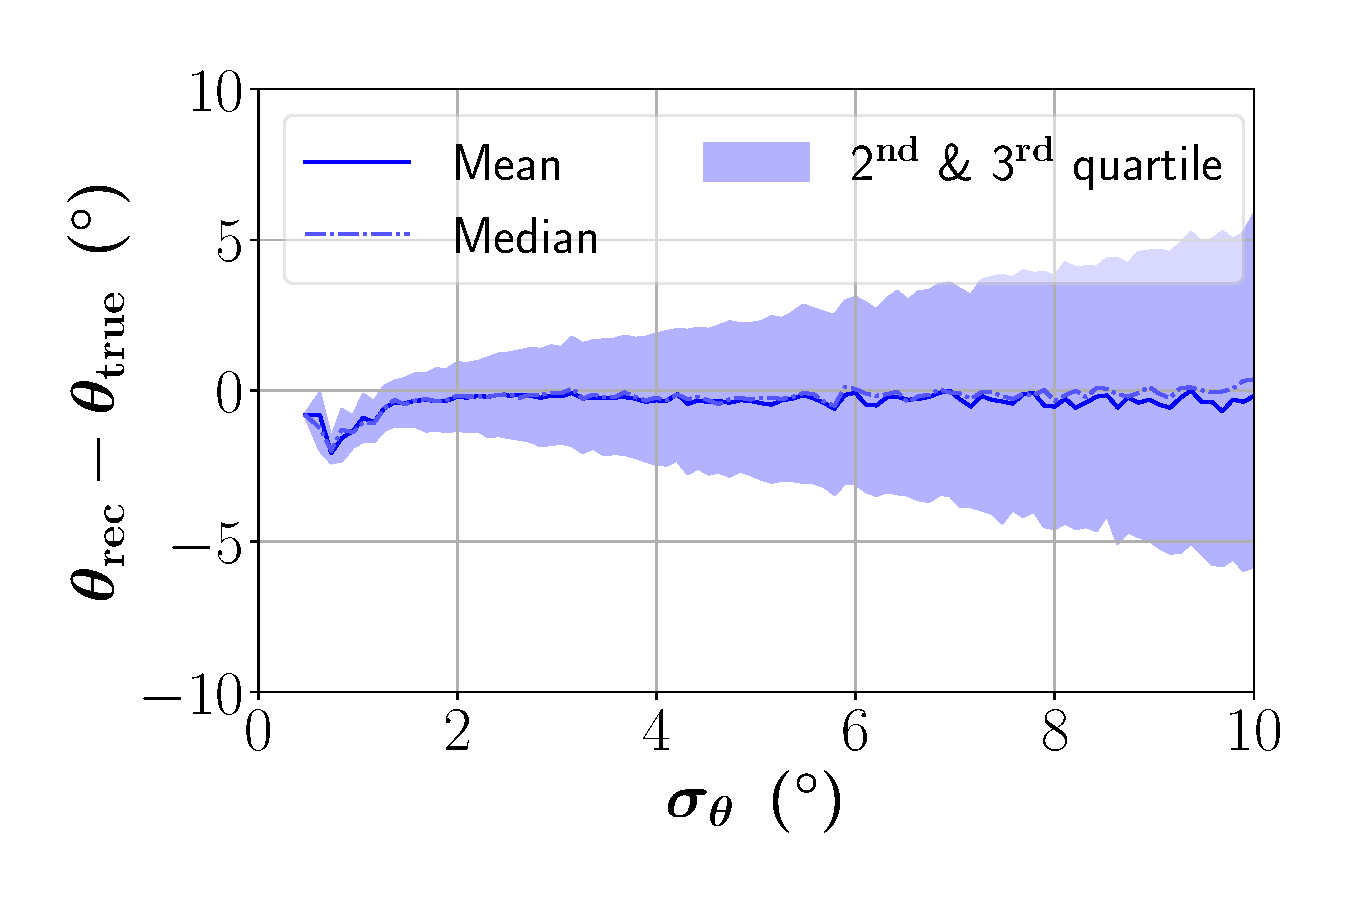
\includegraphics[width=.48\textwidth]{figs2/sigma_Zenith_track}
	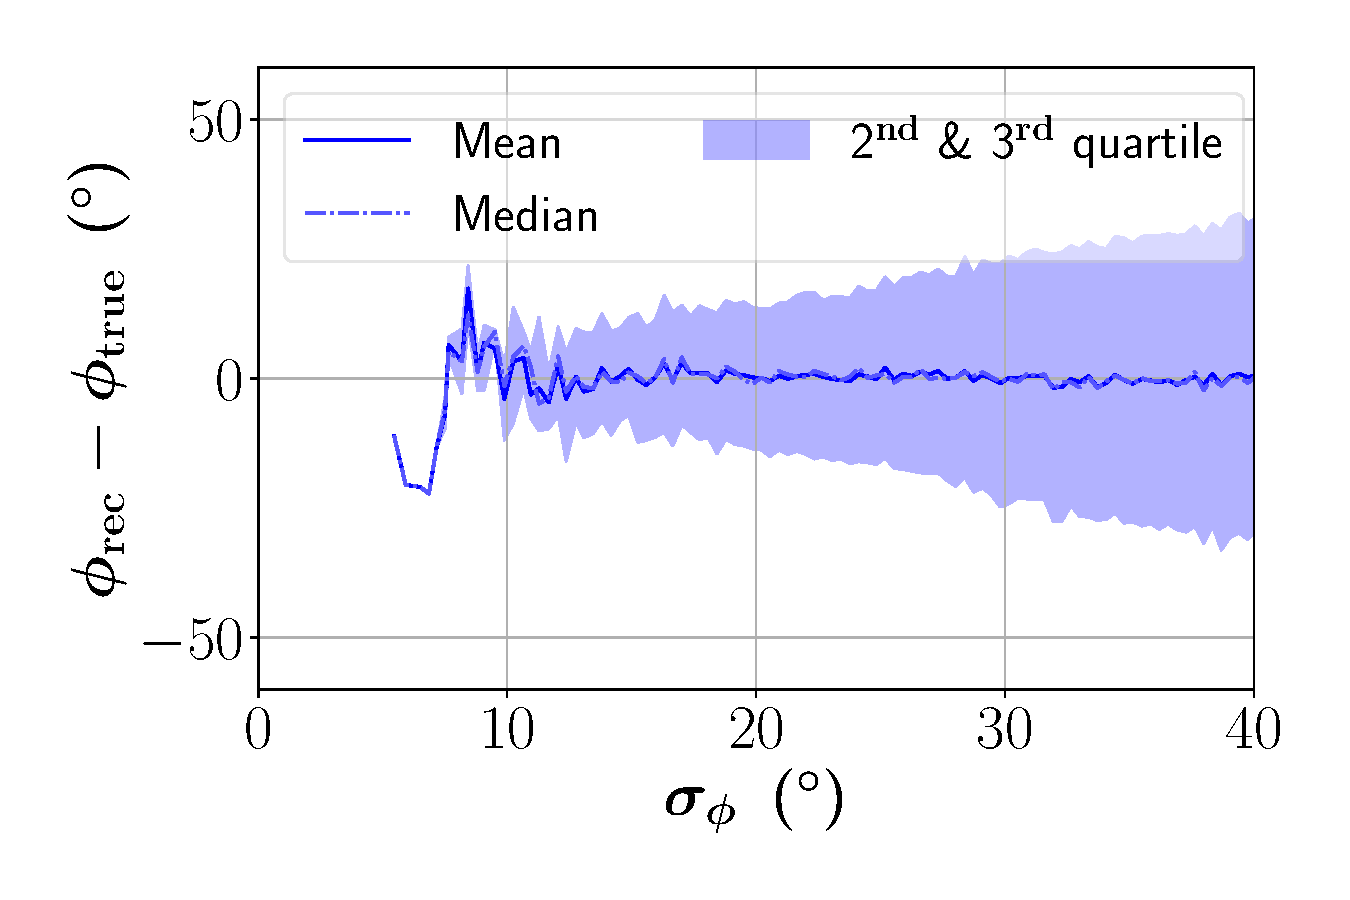
\includegraphics[width=.48\textwidth]{figs2/sigma_Azimuth_track}
	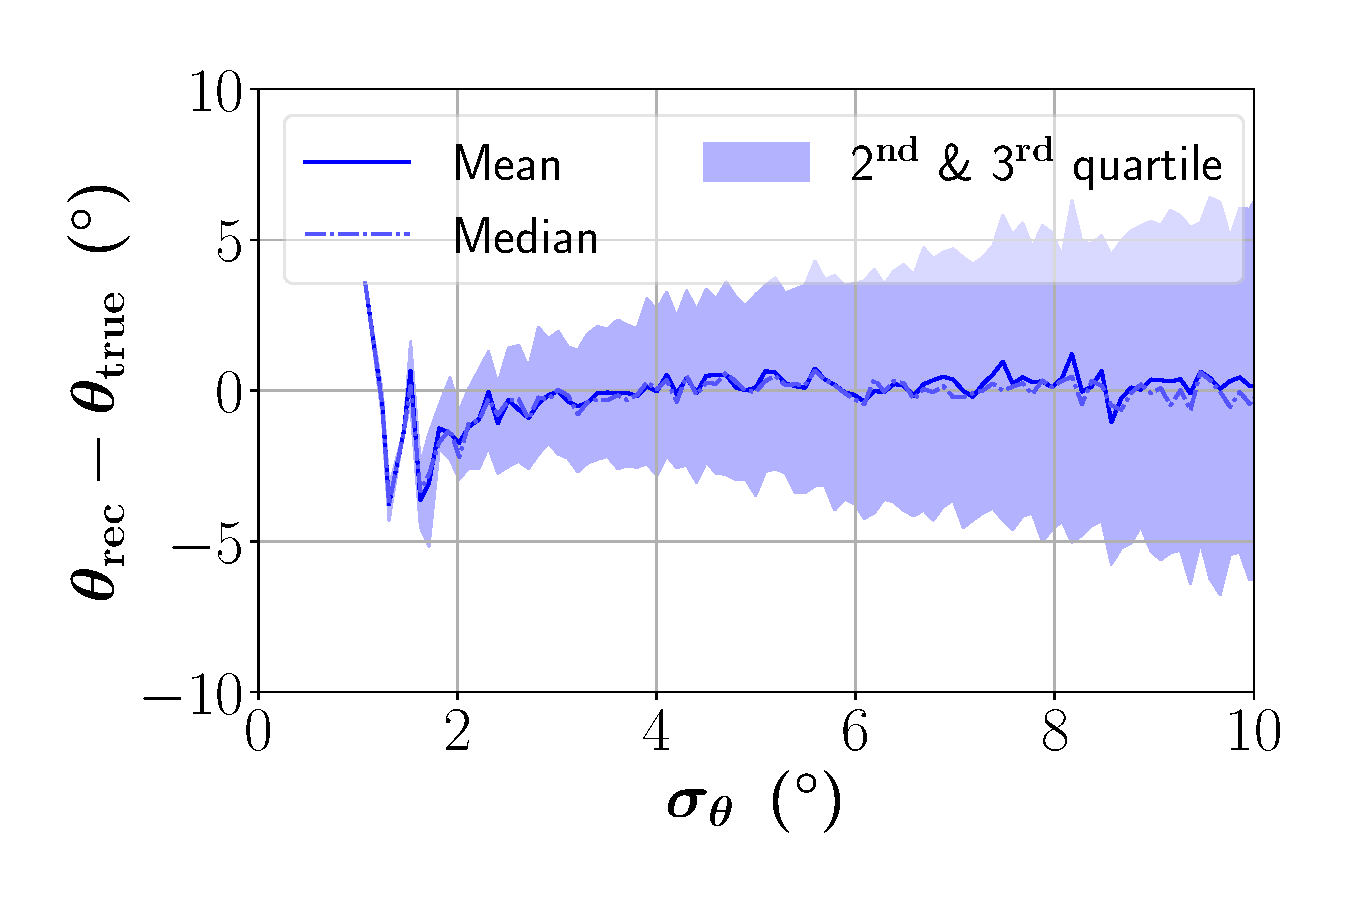
\includegraphics[width=.48\textwidth]{figs2/sigma_Zenith_shower}
	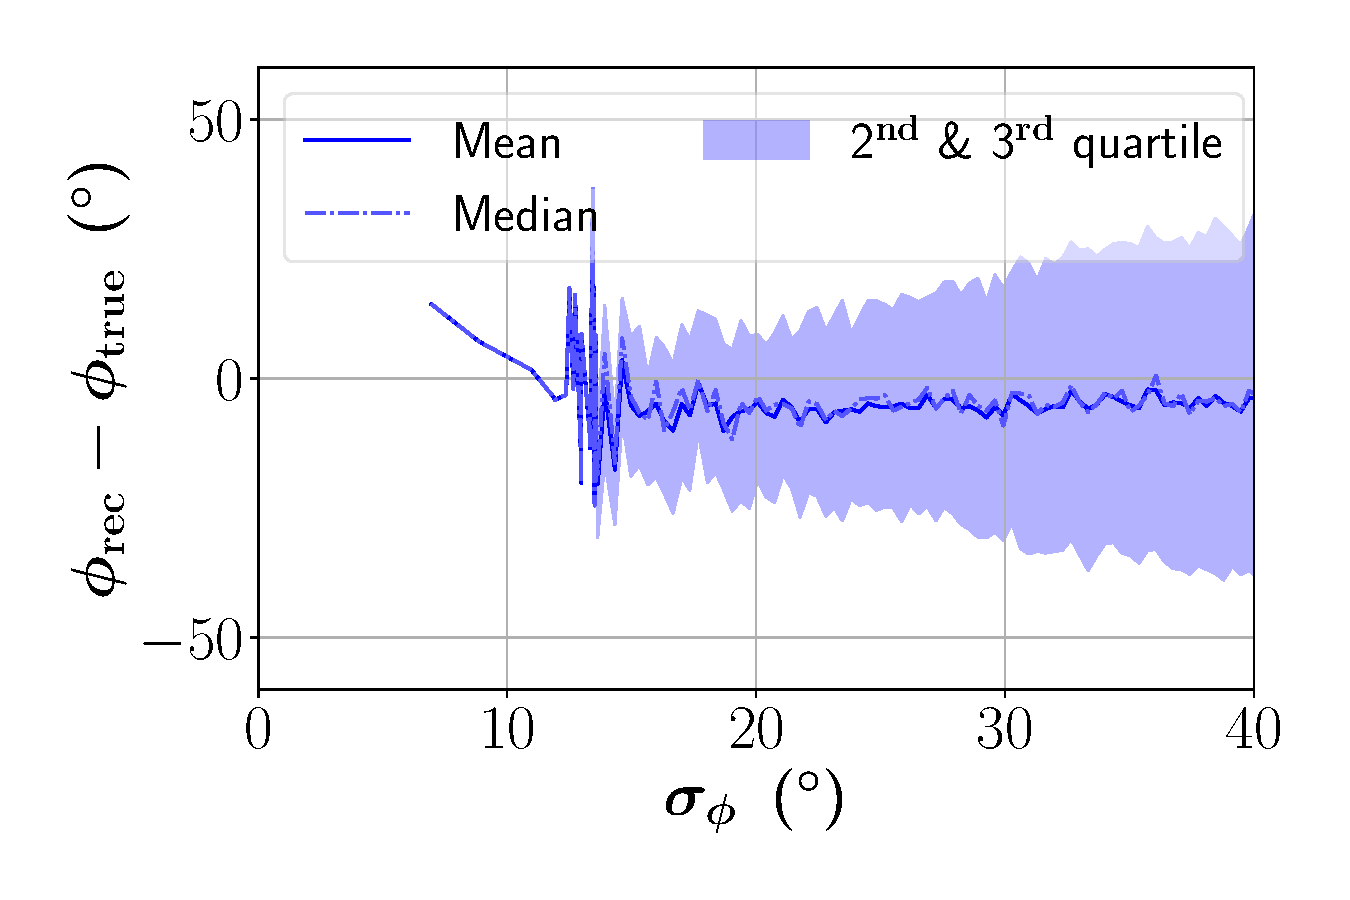
\includegraphics[width=.48\textwidth]{figs2/sigma_Azimuth_shower}
	\caption{\label{fig:sigma}Angles $\theta$ and $\phi$ error as function of the predicted uncertainty for the \textbf{track} (top) and \textbf{shower} (bottom) branches. The mean and median error stay close to zero with no significant bias. Second and third quartiles behave as expected for a Gaussian distribution, especially for $\theta$.}
\end{figure}

%\begin{figure}[htbp]
%	\centering
	
%	\caption{\label{fig:sigma_sh}Angles $\theta$ and $\phi$ error as function of the predicted uncertainty for the \textbf{shower} branch. The mean and median error stay close to zero with no significant bias. Second and third quartiles behave as expected for a Gaussian distribution, especially for $\theta$.}
%\end{figure}



\subsection{Closest point and interaction vertex}
\label{subsec:closest}

%Due to the dependency of the energy deposited in the detector on the distance and position of the event to the lines, we decided to reconstruct these variables before the energy.

In addition to the reconstruction of direction, estimating the energy of neutrino events is fundamental for physics analysis. Energy and distance to the detector are, however, intermingled in SL events: distant high-energy events may appear as SL as much as near low-energy events. Then, to improve the energy estimation, we included in $N$-fit the reconstruction of the \emph{closest point} of track events to the ANTARES detector line, and the \emph{interaction vertex} position of showers events, since these two magnitudes are characterized by the horizontal distance in meters ($R_c$ for closest point of tracks, $R_v$ for interaction vertex of showers) and their vertical position ($Z_c$ for tracks, $Z_v$ for showers) defined in the ANTARES frame of reference.

Independent networks (\autoref{fig:network_RZ}) were used for the horizontal distance ($R$) and vertical coordinate ($Z$). Their architecture was that of the direction reconstruction without further tuning. Differences lay in networks' input and output to fulfil the characteristics of these reconstructions. Thus, events were not centred across images in these network models to ease the reconstruction of $Z$. In addition, these networks also incorporated the reconstruction of $\theta$ as input, which was introduced in parallel to the convolutional layers. Lastly, the loss function, equation (\ref{eq:loss_RZ}), was adapted in consonance with the outputs of these networks: 

\begin{equation}
	\label{eq:loss_RZ}
	\begin{split}
		\mathcal{L} = &\ln (\sqrt{2\pi}\sigma_{R}) + \frac{1}{2}\frac{(R_{t}-\mu_{R} )^2}{\sigma_{R}^2}+\\
		+ &\ln (\sqrt{2\pi}\sigma_{Z}) + \frac{1}{2}\frac{(Z_{t}-\mu_{Z} )^2}{\sigma_{Z}^2}.
	\end{split}
\end{equation}

\begin{figure}[htbp]
	\centering
	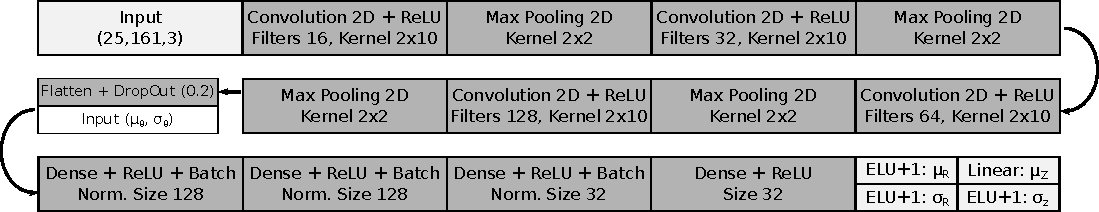
\includegraphics[scale=0.69]{figs2/DCN_RZ.pdf}
	\caption{\label{fig:network_RZ}Details of the closest point and interaction vertex network architecture.}
\end{figure}


\subsection{Energy}
\label{subsec:energy}

As described earlier, estimating the energy is particularly challenging for SL events, especially for track events, given their physical characteristics and the limited information available by a single line of the detector. Shower events are slightly better suited for energy reconstruction because of their physical topology. Moreover, the neutrino energy is directly inferred by $N$-fit in shower events, whereas for track events, the reconstructed energy by $N$-fit is limited to that of the secondary muon. This is due to the stochastic energy loss in neutrino interactions producing track events. The neutrino energy of track events for physics analyses can, however, be inferred indirectly, by combining $N$-fit energy reconstruction and the statistical properties of the interactions.

As a first approximation, we applied the same model architecture of the direction reconstruction to infer energy without further tuning. The energy reconstructions by that model presented very low accuracy. Reasons underlying the poor performance include that the secondary muon can escape the detector in track events, or that events could be very close or far away from the detector line in shower events. To better guide training in the $N$-fit energy reconstruction, we preselected events that we knew had good direction reconstruction (i.e., the events of the 50\% best $\sigma_\theta$), and that we knew that were close to the line (according to the $\{R,Z\}$ reconstruction). The specific cuts appear in expression (\ref{eq:cuts_tr}) for tracks, and in expression (\ref{eq:cuts_sh}) for showers.

\begin{equation}
\setlength{\jot}{10pt}
	\label{eq:cuts_tr}
	\begin{gathered}
		R_c \leq 50\,m~~~~Z_c \in (-150, 150)\,m~~~~\sigma_\theta\leq8.6^\circ\\
		\sigma_{R_c} \leq 4.3\,m~~~~\sigma_{Z_c} \leq 6.2\,m
	\end{gathered}
\end{equation}

\begin{equation}
\setlength{\jot}{10pt}
	\label{eq:cuts_sh}
	\begin{gathered}
		R_v \leq 50\,m~~~~Z_v \in (-150, 150)\,m~~~~\sigma_\theta\leq 14.9^\circ\\
		\sigma_{R_v} \leq 5.6\,m~~~~\sigma_{Z_v} \leq 3.3\,m
	\end{gathered}
\end{equation}

After training with these cuts, energy inference slightly improved. We considered this model as the \textit{benchmark} to evaluate further improvements, particularly that from indirect transfer learning through PCA-based knowledge distillation. In such approach, we aimed to exploit the relationship between the energy of the neutrino and all other physical parameters of the event processed by $N$-fit direction and distance models. We assumed that internal representations from those models could then benefit energy predictions. To test the hypothesis, neuron activations in hidden layers from the $\theta$ and $\{R,Z\}$ networks were taken as feature dimensions from which to infer events' energy. We disregarded, however, activations from the $\phi$ network for two main reasons, first due to the symmetry in $\{X,Y\}$, and second because of the low accuracy of $\phi$ estimations in SL events, compared to $\theta$ and $\{R,Z\}$ estimations.

We linearly transformed all feature dimensions, using the PCA, to rank components according to their variability. We then selected those most relevant features as inputs to a FFN trained to infer the energy as point predictions (\autoref{fig:network_e}). The final number of components, 63 features for the track branch and 68 for the shower branch, was determined applying the elbow rule, i.e., stopping incorporating more features once the cumulated variance reached a \textit{plateau}. Concurrently, we realized that inferring $\log (E)$ performed better than estimating $E$ directly, due to the large energy range of neutrino events (from 5 GeV up to 20 TeV).

In a subsequent phase aimed to further improve energy predictions for physics analyses, we designed a specialized FFN by feeding the model during training only with the 50\% best reconstructions from the original model shown in \autoref{fig:network_e}. In addition, this specialized FFN incorporated a MDN output layer to provide uncertainty estimation of energy predictions, as well as loss weighting factors to balance the impact of the non-uniform energy distribution.

\begin{figure}[htbp]
	\centering
	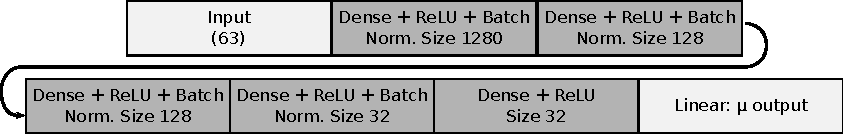
\includegraphics[scale=0.69]{figs2/NNEnergy.pdf}
	\caption{\label{fig:network_e}Details of the energy network architecture.}
\end{figure}

\subsection{Classification}
\label{subsec:class}

$N$-fit includes a neural network for track vs. shower classification, which leverages transfer learning from the specialized track and shower branches. It outputs the probability of an event to be a track ($P$), so the probability of being shower is $1-P$. To train, validate and test the classifier, we used a combined dataset made of 200,000 MC events, half of them representing track events ($\nu_\mu^{CC}$) and the other half representing shower events ($\nu_\mu^{NC}$, $\nu_e^{NC}$, $\nu_e^{CC}$). This new dataset, as well as the previous used in the training phase, are selected according to the $\chi^2$-fit SL criteria with no further refinement. All events were randomly sampled in a uniform manner covering the full period in which ANTARES collected data.

The \emph{control} network model for classification consisted of the same model architecture of the direction reconstruction without further tuning. Only the output was adjusted: a single neuron represented the probability of an event to be a track ($P$), using the sigmoid as its activation function. Given that track and shower events typically present different trace characteristics and that these traits were presumably present as internal representations in the convolutional layers of $N$-fit direction and distance reconstruction models, we decided to exploit this knowledge in a second, more sophisticated classifier endowed with TL. Specifically, we incorporated the convolutional blocks of the $\theta$, $\phi$ and $\{R,Z\}$ network models from both $N$-fit branches as frozen components that were plugged in parallel into a FFN. This network model also incorporated the reconstruction of the energy and its uncertainty from the networks specialized in track and shower events. The complete architecture is shown in \autoref{fig:network_class}.

\begin{figure}[htbp]
	\centering %width=1.\textwidth %scale=0.73
	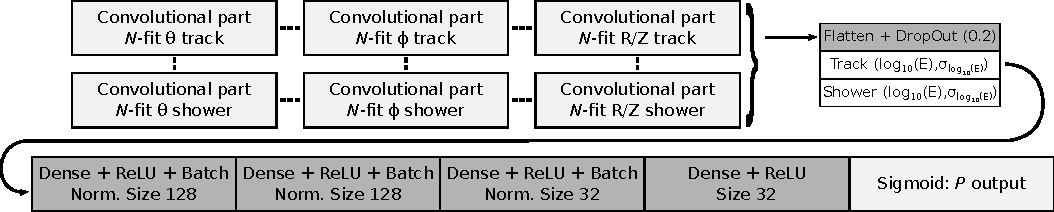
\includegraphics[scale=0.69]{figs2/DCN_class.pdf}
	\caption{\label{fig:network_class}Details of the classifier network architecture. All convolutional blocks are connected in parallel to the feed-forward part.}
\end{figure}

\subsection{Code implementation and computational efficiency}
\label{subsec:code}

All neural network models were implemented using the TensorFlow 2.4.1 framework, with model evaluation and analysis conducted in Python 3.9.15. The implementation relied on standard scientific computing libraries, including \texttt{NumPy 1.23.4}, \texttt{Scikit-learn 1.1.3}, and \texttt{Pandas 1.5.1}, along with several auxiliary packages.

Training times varied depending on network architecture. Specifically, direction and position networks required approximately 12 hours each to train, leveraging GPU acceleration via TensorFlow. Principal Component Analysis, applied separately to each branch (track and shower), required roughly 15 minutes per branch. The subsequent training of the energy reconstruction networks took between 5 and 15 minutes, being much faster than the spatial models primarily due to their lack of convolutional layers, which are typically the most computationally demanding components. Training the track vs. shower classifier, which reuses frozen convolutional layers transferred from the specialized branches, was comparatively lightweight, requiring only about 20 minutes. GPU-accelerated training was conducted on a workstation running KDE Neon 24.04, equipped with two NVIDIA Quadro RTX 8000 GPUs (TU102GL architecture, 64-bit interface), each of them having a 48 GB GDDR6 memory and supporting 672 GB/s memory bandwidth. % The system used the proprietary NVIDIA driver and was accessed via a KDE Neon 24.04 environment.

%All training and testing procedures were executed on a small server... \notaJGM{@Salva, ¿Puedes dar detalles del hardware, GPU, CPU, RAM, y software?}

The final application of the $N$-fit algorithm to ANTARES data was organized into three main phases: (i) reading the ANTARES data files, (ii) processing the raw data into the standardized $N$-fit input format, and (iii) performing the actual reconstruction. The first phase is common to any reconstruction pipeline and does not affect the evaluation of $N$-fit's computational performance. The image generation stage, where detector hits are transformed into 2D representations for network input, took on average 0.2 seconds per event. The complete reconstruction process required approximately 0.1 seconds per event. These estimates are based on the averaged processing times over 10,000 events, using conservative rounding to ensure upper-bound accuracy. In both cases, model parameters and dependencies were preloaded into memory cache, eliminating the overhead of repeated I/O operations during batch processing.

The whole application of $N$-fit to the ANTARES data was executed on the high-throughput computing (HTC) partition of the IN2P3 Computing Center, managed via the SLURM workload manager. The HTC partition consists of heterogeneous CPU-only nodes running Red Hat Enterprise Linux release 9.6 (64-bit). Most nodes are equipped with AMD EPYC 7302 16-core, EPYC 7453 28-core, or EPYC 9334 32-core processors, with memory per node ranging from 192~GB to over 1.2~TB. For our runs, a single CPU core and less than 2~GB of RAM were sufficient for efficient reconstruction inference. GPU resources were not required for deployment, although training leveraged TensorFlow's GPU acceleration when available.


%\notaSA{Dado que, como dice Juan, (1) los datos de ANTARES a nivel de hits están disponibles solo para la colaboración, y que (2) también existen limitaciones sobre código ANTARES, pero como (3) ANTARES ya ha concluido su labor, al menos en lo que respecta a la toma de nuevos datos; me parece que le deberíamos comentar a la comisión interna de revisión del manuscrito sobre la disponibilidad en abierto del (a) código y/o (b) los datos que se han usado, en algún repositorio público que podamos referenciar en el manuscrito; según su respuesta, las referencias se añadirían aquí, o no.}

% -------------------------------------------------------
% For the marker to be outside last chapter when using bookmarks in an electronic PDF
\bookmarksetup{startatroot}

\phantomsection
\chapter*{Conclusions}
\markboth{Conclusions}{Conclusions}
\addcontentsline{toc}{chapter}{Conclusions}
\label{chap:conclusions}

This thesis has addressed three complementary aspects of modern astroparticle physics: the use of neutrinos as cosmic messengers, the application of machine learning to enhance detector performance, and the search for dark matter through neutrino observations of the Sun. The results obtained provide both methodological advances and physics insights, while also pointing to promising directions for future work.

\phantomsection
\section*{Summary of Contributions}
\addcontentsline{toc}{section}{Summary of Contributions}

In the first part of this manuscript, the foundations of neutrino astronomy and the ANTARES telescope were introduced. These chapters set the framework for the subsequent developments, emphasizing both the potential and the challenges of neutrino telescopes as tools for fundamental physics.

The second part of this thesis was dedicated to the development of a new machine learning--based reconstruction algorithm, \textbf{\textit{N}-fit}, specifically designed to improve the treatment of single-line events in ANTARES. Using deep convolutional architectures, mixture density outputs, and transfer learning, $N$-fit achieves a significant reduction in angular reconstruction errors. For track-like events, the mean $\theta$ error decreased from $\sim 9.7^\circ$ (standard $\chi^2$-fit) to $\sim 3.7^\circ$ for the best 50\% quality parameters. The method also provides, for the first time in ANTARES, an azimuthal estimate for single-line events, with a mean error of $\sim 29.2^\circ$ for the best 50\% events according to the predicted uncertainty in the direction. The algorithm also improved distance and vertex reconstruction, enabling better constraints on the geometry of the interaction with respect to the detector; and enhanced energy reconstruction, particularly for shower-like events, where transfer learning allowed a reduction of the energy error compared to baseline models. The explicit estimation of uncertainties in every reconstructed property makes it possible to select subsets of events with robust predictions. Last but not least, a track-vs-shower classifier is presented with an accuracy of $\sim 80\%$, demonstrating the ability of transfer learning to leverage specialized feature extractors across tasks. When comparing data and MC simulations, $N$-fit demonstrates a good agreement in the tracks branch, cleaning the background noise and atmospheric muons of the up-going sample when quality cutoffs are applied.

All together, these results show that machine learning can substantially extend the physics reach of ANTARES by unlocking information from previously underutilized event classes. Beyond ANTARES, the methodology and architecture of N-fit may be transferable to current and future neutrino telescopes, such as KM3NeT.

The third part of this thesis focused on a physics application: the search for dark matter signals from the Sun. Building on the methodological advances, an unbinned maximum likelihood analysis was performed using the full ANTARES dataset. The analysis included the generation of probability density functions, pseudo-experiments, and sensitivity studies across a wide range of WIMP masses. No significant excess of neutrino events from the direction of the Sun was observed. Thus, upper limits were placed on the neutrino flux from WIMP self-annihilation in the Sun, for different annihilation channels and WIMP masses ranging from a few GeV to a few TeV. These limits translate into constraints on the spin-dependent and spin-independent WIMP-nucleon scattering cross section that are complementary to, and at some points competitive with, those obtained from direct detection experiments.

\phantomsection
\section*{Discussion}
\addcontentsline{toc}{section}{Discussion}

The developments presented in this thesis illustrate the synergy between new data analysis techniques and fundamental physics goals. On the methodological side, the implementation of deep learning in $N$-fit demonstrates that artificial intelligence can provide not only incremental but qualitative improvements in reconstruction, opening analysis channels that were previously inaccessible. On the physics side, the dark matter search conducted with ANTARES data contributes to the global effort of constraining the parameter space of WIMPs, probing scenarios that are difficult to test with laboratory-based experiments.

A direct comparison with other experiments highlights the complementarity of the results. In the region of high WIMP masses ($\gtrsim 1$ TeV), ANTARES constraints on the spin-dependent WIMP-nucleon scattering cross section are comparable to those from IceCube, benefitting from the different geographical location and analysis strategies. %At lower WIMP masses (tens to hundreds of GeV), ANTARES results are competitive with those of Super-Kamiokande, despite its smaller instrumented volume, thanks to optimized reconstruction and background suppression.
When contrasted with direct detection experiments such as PICO, LUX-ZEPLIN, or XENONnT, the ANTARES limits are weaker in the spin-independent channel, but provide unique sensitivity to the spin-dependent channel where neutrino telescopes probe parameter space that is otherwise inaccessible. This underlines the complementarity of direct, indirect, and collider searches: only by combining them can the full range of possible dark matter scenarios be tested.

One important lesson emerging from this work is the role of uncertainty estimation. Both in the reconstruction tasks and in the physics analyses, the ability to assign reliable confidence measures to predictions is crucial for building robust likelihood functions and for maximizing sensitivity. This aspect is expected to become even more relevant in the era of larger detectors and more complex datasets.

\phantomsection
\section*{Future Prospects}
\addcontentsline{toc}{section}{Future Prospects}

Looking ahead, several avenues for further research arise naturally from this work.Future versions of N-fit could explore more advanced neural architectures, such as attention mechanisms or graph neural networks, which may better capture the sparse and relational structure of neutrino telescope data. Joint training across multiple tasks (direction, energy, classification) could further enhance performance. Furthermore, the experience gained with $N$-fit on ANTARES data is directly applicable to KM3NeT, whose larger volume and denser instrumentation will benefit from advanced machine learning reconstruction. In particular, the ability to reconstruct events with improved accuracy is central for oscillation studies in ORCA and point-source searches in ARCA.

On the dark matter side, the limits obtained can be extended by combining results from ANTARES with other telescopes in joint analyses. Moreover, $N$-fit can be exploited in other contexts, such as neutrino physics measurements or transient source searches, where the inclusion of single-line events can significantly boost statistics.

\phantomsection
\section*{Concluding Remarks}
\addcontentsline{toc}{section}{Concluding Remarks}

In conclusion, this thesis has shown how innovative reconstruction methods based on deep learning can open new possibilities in neutrino astronomy and physics, and how these tools can be harnessed to address one of the most pressing questions in physics: the nature of dark matter. The methods and results presented here provide a foundation for future discoveries, particularly with the new generation of neutrino telescopes, and exemplify the fruitful intersection of artificial intelligence and fundamental science.



% -------------------------------------------------------
% -------------------------------------------------------
% -------------------------------------------------------
% Apéndices de la publicación
\part*{Appendix}
\appendix

\chapter{Brief mathematical demonstrations}

\clearpage
\section{Differential equation solution for the number of WIMPs in the Sun}
\label{app:diff}

Take this expression:

\begin{equation}
	\frac{\mathrm{d}N}{\mathrm{d}t} = C_\odot - A_\odot \cdot N^2.
\end{equation}

Splitting the terms which depend on $N$ and $t$, we get:

\begin{equation}
	\frac{\mathrm{d}N}{C_\odot - A_\odot \cdot N^2} = \mathrm{d}t.
\end{equation}

Now, integrating in both sides, from $t_0 = 0$, when $N(t_0) = 0$, to the age of the Solar System $t_\odot$:

\begin{equation}
	\label{eq:int}
	\int_0^N \frac{1}{C_\odot - A_\odot \cdot N^2} \,\mathrm{d}N = \int_{0}^{t_\odot} \mathrm{d}t.
\end{equation}

Focusing on the left integral, we can write it as:

\begin{equation}
	\int_0^N \frac{1/C_\odot}{1 - A_\odot/C_\odot \cdot N^2} \, \mathrm{d}N .
\end{equation}

We now can make a variable change, such that:

\begin{equation}
	\left.
	\begin{aligned}
		N &= \sqrt{C_\odot/A_\odot} \cdot \tanh(x)\\
		x &= \textrm{arc}\tanh\left(\sqrt{A_\odot/C_\odot} \cdot N\right)  
	\end{aligned} \right\}
	\Longrightarrow \mathrm{d}N = \sqrt{C_\odot/A_\odot} \cdot \left(1-\tanh^2(x)\right)\, \mathrm{d}x.
\end{equation}

Thus, we can re-write and solve the integral:

\begin{equation}
	\begin{aligned}
	\int_0^N \frac{1/C_\odot}{1 - A_\odot/C_\odot \cdot N^2} \, \mathrm{d}N =&
	\int_0^x \frac{1/C_\odot \cdot  \sqrt{C_\odot/A_\odot}  \cdot  \left(1-\tanh^2(x)\right)}{1-A_\odot/C_\odot  \cdot \left( \sqrt{C_\odot/A_\odot} \cdot \tanh(x) \right)^2} \, \mathrm{d}x =  \\
	=& \int_0^x \frac{1/\sqrt{A_\odot C_\odot}  \cdot  \left(1-\tanh^2(x)\right)}{1- \tanh^2(x)} \, \mathrm{d}x = \\
	=& \int_0^x 1/\sqrt{A_\odot C_\odot} \, \mathrm{d}x = \\
	=& \,x/\sqrt{A_\odot C_\odot}.
	\end{aligned}
\end{equation}

Undoing the variable change and introducing the result in equation \ref{eq:int}:

\begin{equation}
	\begin{gathered}
		\textrm{arc}\tanh\left(\sqrt{A_\odot/C_\odot} \cdot N\right) /  \sqrt{A_\odot C_\odot} = t_\odot \Longrightarrow \\
		\Longrightarrow \textrm{arc}\tanh\left(\sqrt{A_\odot/C_\odot} \cdot N\right) = \sqrt{A_\odot C_\odot} \cdot t_\odot \Longrightarrow \\
		\Longrightarrow \boxed{ N = \sqrt{C_\odot/A_\odot} \cdot \tanh\left(\sqrt{A_\odot C_\odot} \cdot t_\odot \right)}
	\end{gathered}
\end{equation}

With this result and using that $A_\odot N^2$ is twice the annihilation rate $\Gamma_\odot$ by definition, we can conclude that:

\begin{equation}
	\begin{gathered}
		\Gamma_\odot = \frac{1}{2}A_\odot N^2 = \frac{1}{2}A_\odot \cdot \frac{C_\odot}{A_\odot} \cdot \tanh^2\left(\sqrt{A_\odot C_\odot} \cdot t_\odot \right) \Longrightarrow \\
		\Longrightarrow \boxed{\Gamma_\odot = \frac{1}{2} C_\odot \cdot \tanh^2\left(\sqrt{A_\odot C_\odot} \cdot t_\odot \right)},
	\end{gathered}
\end{equation}

as we wanted to demonstrate.

% -------------------------------------------------------
% -------------------------------------------------------
% -------------------------------------------------------
% Bibliografía

\bibitemsep = 3ex
\bibhang = 2em
\bookmarksetup{startatroot}
% To avoid over-flux. It causes under-flux, but it is preferable. Start with it commented and play with the number
\emergencystretch=1.5em
\printbibliography[heading=bibintoc,title=\bibname]

% -------------------------------------------------------
% Índice alfabético

%\cleardoublepage
%\phantomsection
%\addcontentsline{toc}{chapter}{\indexname}
%\printindex

% -------------------------------------------------------
% Fin del documento

\end{document}

% ---------------------------------------------------------------------
% ---------------------------------------------------------------------
% ---------------------------------------------------------------------